
\markedchapter{Count Data Example}{Worked Example without Distance Sampling}
\label{cha:near}
%~~~~~~~~~~~~~~~~~~~~~~~~~~~~~~~~~~~~~~~~~
%~~~~~~~~~~~~~~~~~~~~~~~~~~~~~~~~~~~~~~~~~~~
\section{Introduction} 
\begin{frame}
This chapter takes you through the process of fitting spatial models using the CReSS method in a GEE framework with SALSA for model selection (section \ref{sec:nsmodfit}).  We use simulated vantage point data as our case study.  Section \ref{sec:nspreds} uses the fitted count model to make predictions across the entire study area, which we use to draw inference from our study. We use simulated vantage point data as our case study.  The type of impact was a redistribution of animals within the study area. 

\begin{block}{Aim}
Produce a density surface map along with estimates of uncertainty and identify any significant effect of an event (e.g. nearshore renewable installation).
\end{block}

\noindent Note: No distance sampling analysis can be conducted as there is no information available to do so.

\noindent The following sections take you through:

\begin{itemize}
  \item model fitting 
  \item checking diagnostics
  \item making predictions and inference
\end{itemize}

\end{frame}


%~~~~~~~~~~~~~~~~~~~~~~~~~~~~~~~~~~~~~~~~~
%~~~~~~~~~~~~~~~~~~~~~~~~~~~~~~~~~~~~~~~~~~~

\markedsection{Preparation}{Preparing to conduct an analysis with MRSea} 
Before we start, we load the {\tt MRSea} package and its dependencies. 
This may require installing the following packages if they are not already installed on your computer: 
\begin{itemize}
\item mrds, lawstat, car, mvtnorm, splines, geepack, ggplot2, calibrate, Matrix and fields.
\end{itemize}
After installing these packages, the following command will load package {\tt MRSea} and these packages into the active workspace. \\

\noindent See section \ref{sec:mrseadata} for information on the datasets this package holds.

%~~~~~~~~~~~~~~~~~~~~~~~~~~~~~~~~~~~~~~~~~
%~~~~~~~~~~~~~~~~~~~~~~~~~~~~~~~~~~~~~~~~~~~
\section{Loading the Data}

\subsection{Data Requirements}
There are a few requirements for analysing data using the {\tt MRSea} package.

\begin{itemize}
\item The geographic coordinates must be labelled {\tt x.pos} and {\tt y.pos}
\item There must be a column labelled {\tt area} representing the effort associated with each coordinate
\end{itemize}

\begin{frame}[fragile]
\begin{knitrout}\footnotesize
\definecolor{shadecolor}{rgb}{0.969, 0.969, 0.969}\color{fgcolor}\begin{kframe}
\begin{alltt}
\hlcomment{# Loading the data}
\hlfunctioncall{data}(\hlstring{ns.data.re})
data <- ns.data.re
\hlfunctioncall{attach}(data)
\hlfunctioncall{head}(data, n=3)
\end{alltt}
\begin{verbatim}
  x.pos y.pos   area  floodebb observationhour GridCode Year
1  1500 -4500 0.3853       EBB              12      a11    9   
2  1500 -4500 0.3853     FLOOD               8      a11    9    
3  1500 -4500 0.3853     FLOOD               9      a11    9   

  DayOfMonth MonthOfYear impact  birds cellid
1         13           3      0      0      1
2         16           3      0      0      2
3         16           3      0      0      3
\end{verbatim}
\end{kframe}
\end{knitrout}
\end{frame}

\subsection{Exploratory Data Analysis (EDA)}

\begin{frame}[fragile]
Assess the data inputs for the modelling process. 
\begin{itemize}
\item Check for unusual covariate values
\item Identify possible relationships between covariates and the response (animal counts)
\item This data was collected by a cliff-top observer (grey dot, Figure \ref{fig:gridcells})
\end{itemize}


\begin{figure}[h!]
  \centering
  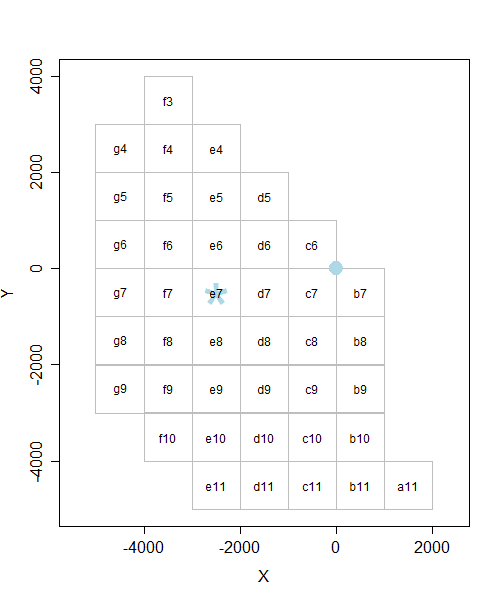
\includegraphics[width=6cm]{bc/vpgridcells.png}
\caption{Grid cell identifiers for the study region.  The grey circle is the location of a cliff-top observer and the star the site of the impact event.}
\label{fig:gridcells}
\end{figure}
\end{frame}

\begin{frame}
\begin{figure}[h!]
\centering
  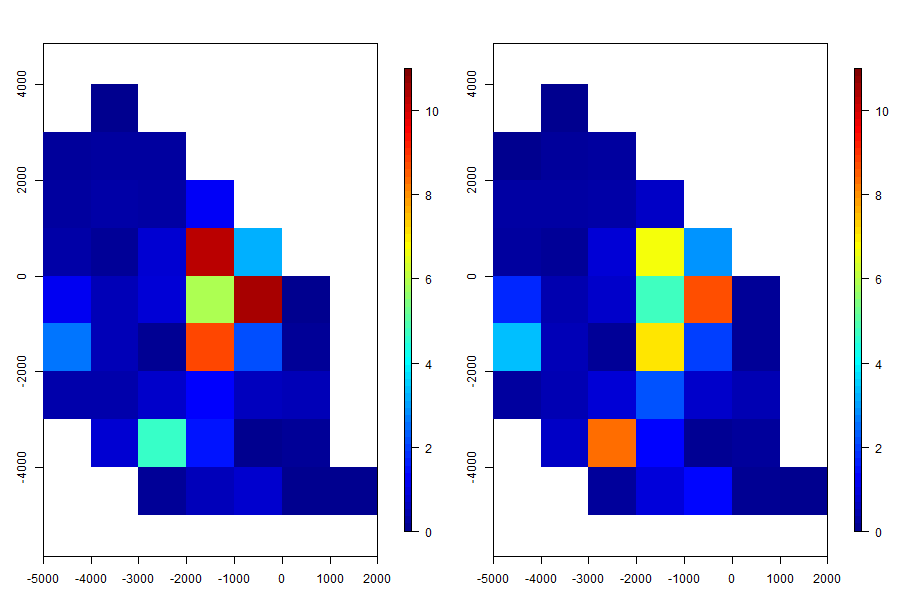
\includegraphics[width=9cm]{bc/birds.png}
\caption{Estimated bird counts before (left) and after (right) an impact event.  Each cell is 1 km$^2$ and the colour represents bird count.}
\label{fig:rawnhats}
\end{figure}
\end{frame}

\begin{itemize}
\item Most animals are seen near to the observer (Figure \ref{fig:rawnhats})
\item Few are seen to the far right and far left of the observer
\end{itemize}


\begin{frame}
Assessing the relationships of available covariates and our response (animal counts).
\end{frame}
\begin{frame}
\begin{figure}[h!]
  \centering
  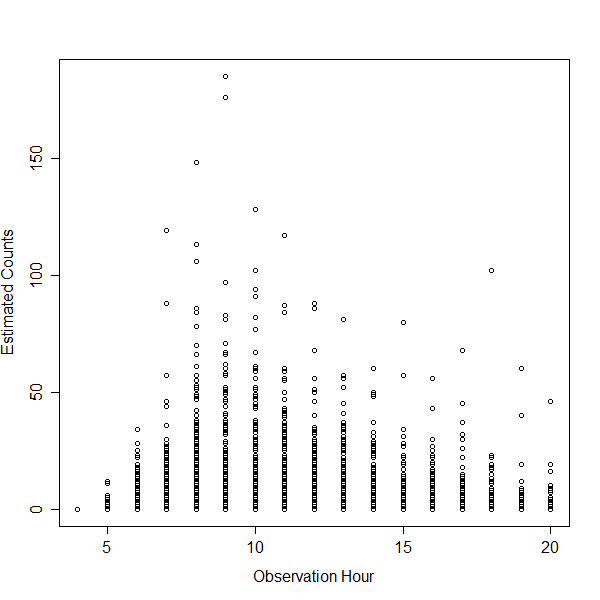
\includegraphics[width=7cm]{bc/obshour.png}
\caption{Plot of observation hour against the estimated bird counts.}
\label{fig:nsexploratory1}
\end{figure}
\end{frame}

\begin{frame}
\begin{figure}[h!]
  \centering
  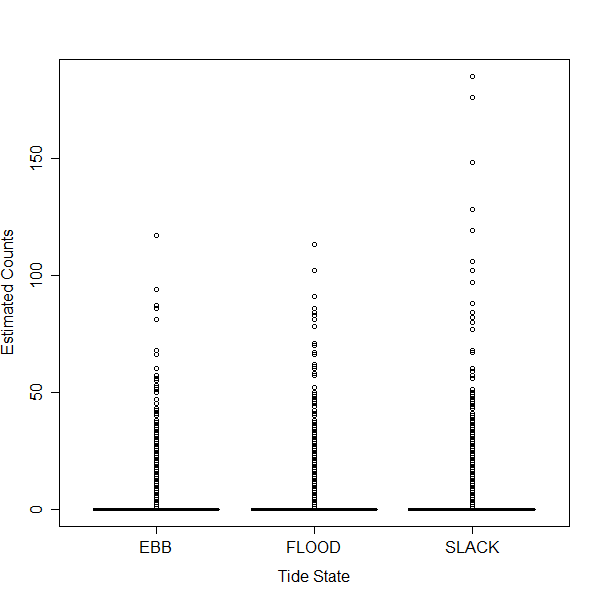
\includegraphics[width=7cm]{bc/floodebb.png}
\caption{Plot of tide state against the estimated bird counts.}
\label{fig:nsexploratory2}
\end{figure}
\end{frame}
\begin{frame}
\begin{figure}[h!]
  \centering
  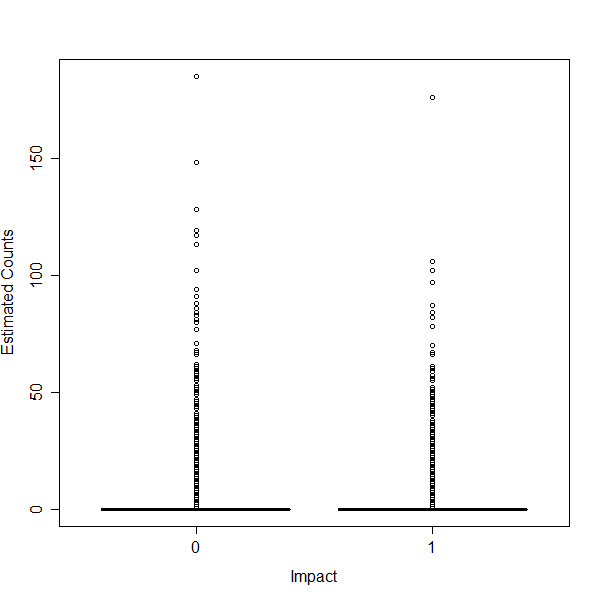
\includegraphics[width=7cm]{bc/impact.png}
\caption{Plot of Impact against the estimated bird counts. Zero is pre impact and one is post impact.}
\label{fig:nsexploratory3}
\end{figure}
\end{frame}


\begin{frame}
\frametitle{EDA}
\begin{itemize}
\item Birds were seen predominantly in the morning hours (7-12).
\item Few birds were seen very early and very late.  
\item Non-linear relationship between observation hour and bird counts.  
\item Difficult to identify any relationship between tide state/impact and bird counts due to the large number of zeros in the data (Figures \ref{fig:nsexploratory2} \&  \ref{fig:nsexploratory3})..
\end{itemize}
\end{frame}
%~~~~~~~~~~~~~~~~~~~~~~~~~~~~~~~~~~~~~~~~~
%~~~~~~~~~~~~~~~~~~~~~~~~~~~~~~~~~~~~~~~~~~~
\clearpage
\subsection{Checking for Collinearity}

\begin{frame}[fragile]
\begin{block}{Variance Inflation Factors (VIFs)}
These are used to assess collinearity between covariates and to tell us by how much the standard error is inflated by the other variables in the model.  For more details see section \ref{subsec:vifs} or  \citet{Fox2011}.
\end{block}

% \begin{itemize}
% \item Generalised VIFs (GVIFs) are calculated, because the covariates have more than one degree of freedom, and adjusted (GVIF$_{\textrm{adj}}$ = GVIF$^{1/2*Df}$) for the number of degrees of freedom.
% \item GVIF$_{\textrm{adj}}$ gives us the decrease in precision of estimation due to collinearity (equivalent to $\sqrt{VIF}$). 
% \item For example, a GVIF$_{\textrm{adj}}$ of 2 means that the confidence intervals are twice as wide as they would be for uncorrelated predictors.
% \end{itemize}
 \end{frame}

\begin{frame}[fragile]
\begin{knitrout}\footnotesize
\definecolor{shadecolor}{rgb}{0.969, 0.969, 0.969}\color{fgcolor}\begin{kframe}
\begin{alltt}
fullModel <- \hlfunctioncall{glm}(birds ~ \hlfunctioncall{as.factor}(floodebb) + \hlfunctioncall{as.factor}(impact) + 
    observationhour + x.pos + y.pos, family = poisson, data = data)
\hlfunctioncall{vif}(fullModel)
\end{alltt}
\begin{verbatim}
                     GVIF Df GVIF^(1/(2*Df))
as.factor(floodebb) 1.006  2           1.002
as.factor(impact)   1.000  1           1.000
observationhour     1.006  1           1.003
x.pos               1.323  1           1.150
y.pos               1.323  1           1.150
\end{verbatim}
\end{kframe}
\end{knitrout}


\begin{knitrout}\footnotesize
\definecolor{shadecolor}{rgb}{0.969, 0.969, 0.969}\color{fgcolor}\begin{kframe}
\begin{verbatim}
[1] "Maximum VIF is: 1.15"
\end{verbatim}
\end{kframe}
\end{knitrout}


\begin{block}{Conclusion:}
The maximum VIF is approximately 1, which means that there is no issue with collinearity (no inflation of standard errors).
\end{block}
\end{frame}


\begin{frame}[fragile]
\frametitle{Checking Factor Covariates}
Each level of a factor-based covariate must have some non-zero entries for the response variable, otherwise there will be problems in the model fitting process 
\begin{knitrout}\footnotesize
\definecolor{shadecolor}{rgb}{0.969, 0.969, 0.969}\color{fgcolor}\begin{kframe}
\begin{alltt}
\hlcomment{# check all factor levels have counts}
\hlfunctioncall{checkfactorlevelcounts}(factorlist=\hlfunctioncall{c}(\hlstring{"floodebb"}, \hlstring{"impact"}), data, data$birds)
\end{alltt}
\begin{verbatim}
[1] "floodebb will be fitted as a factor variable; there are non-zero counts
 for all levels"
[1] "impact will be fitted as a factor variable; there are non-zero counts
 for all levels"
\end{verbatim}
\end{kframe}
\end{knitrout}


\noindent Conclusion: tide state and impact are fine for use in the model.

\end{frame}
%~~~~~~~~~~~~~~~~~~~~~~~~~~~~~~~~~~~~~~~~~
%~~~~~~~~~~~~~~~~~~~~~~~~~~~~~~~~~~~~~~~~~~~
\section{Fitting a Model}
\label{sec:nsmodfit}

\begin{frame}
Here we are going to fit a GEE-CReSS model with SALSA for knot selection. Recap:
\begin{block}{Generalised Estimating Equations (GEE)}
Framework to allow for correlated errors. For more details see \citet{Hardin2002}.
\end{block}

\begin{block}{Complex Region Spatial Smoother (CReSS)}
Flexible spatial smoothing method. For more details see \citet{ScottH2013}.
\end{block}

\begin{block}{Spatially Adaptive Local Smoothing Algorithm (SALSA)}
Automated knot selection procedure for both one-dimensional (e.g. depth) and two-dimensional (e.g. spatial) covariates. The knots are sources of flexibility in the surface that can raise or lower the surface.  For more details see \citet{Walker2010}.
\end{block}
\end{frame}

\subsection{Fitting a Smooth Term}

\begin{frame}[fragile]
\frametitle{A smooth of observation hour}

Construct an object ({\tt splineParams}) that contains the information required by SALSA for adaptive knot placement.
\begin{itemize}
\item Each covariate considered smooth is a list entry in {\tt splineParams} and identified in {\tt varlist}
\item Other inputs include the data and, optionally, a grid of prediction data.
\item The list contains the covariate name, data, initial knot location (one knot at the mean), the boundary knots (greatest range of the prediction data and {\tt data}) and the degree of the smooth.
\item Note:  The smooth one dimensional covariates appear in the {\tt splineParams} object starting at slot {\tt [[2]]}. Slot {\tt [[1]]} is reserved for the spatial term.
\end{itemize}

\begin{knitrout}\footnotesize
\definecolor{shadecolor}{rgb}{0.969, 0.969, 0.969}\color{fgcolor}\begin{kframe}
\begin{alltt}
\hlcomment{# load prediction data}
\hlfunctioncall{data}(ns.predict.data.re)
\hlcomment{# re-named for easier writing}
predictData<-ns.predict.data.re

\hlcomment{# make splineParams object}
splineParams<-\hlfunctioncall{makesplineParams}(data=data, varlist=\hlfunctioncall{c}(\hlstring{'observationhour'}),
         predictionData=predictData)
\hlfunctioncall{str}(splineParams)
\begin{verbatim}
List of 2
 $ : list()
 $ :List of 5
  ..$ covar      : chr "observationhour"
  ..$ explanatory: int [1:27798] 12 8 9 10 11 12 13 14 15 8 ...
  ..$ knots      : num 12
  ..$ bd         : num [1:2] 4 20
  ..$ degree     : num 2
\end{verbatim}
\end{alltt}
\end{kframe}
\end{knitrout}
\end{frame}


\subsection{Checking for Correlation}

\begin{knitrout}\footnotesize
\definecolor{shadecolor}{rgb}{0.969, 0.969, 0.969}\color{fgcolor}\begin{kframe}
\begin{alltt}
fullModel <- \hlfunctioncall{glm}(birds ~ \hlfunctioncall{as.factor}(floodebb) + \hlfunctioncall{as.factor}(impact) + 
    \hlfunctioncall{bs}(observationhour, knots = splineParams[[2]]$knots) + x.pos + y.pos, 
    family = quasipoisson,  data = data)
\end{alltt}
\end{kframe}
\end{knitrout}


\begin{frame}[fragile]
We fit a model containing all covariates of interest ({\tt fullModel} above) and carry out some \textbf{runs tests} to check for \textbf{correlated residuals} (model assumes uncorrelated residuals).

\begin{block}{Runs Test}
This is a test for randomness and allows us to determine if we have correlation in our model residuals. We will see a large $p$-value (H$_0$: uncorrelated residuals) and good mixing of the profile plot if there is no correlation.
\end{block}

\end{frame}


\begin{frame}[fragile]
\noindent The {\tt runs.test} function can be found in the {\tt lawstat} library.
\begin{knitrout}\footnotesize
\definecolor{shadecolor}{rgb}{0.969, 0.969, 0.969}\color{fgcolor}\begin{kframe}
\begin{alltt}
\hlfunctioncall{runs.test}(\hlfunctioncall{residuals}(fullModel, type = \hlstring{"pearson"}), alternative = \hlfunctioncall{c}(\hlstring{"two.sided"}))
\end{alltt}
\begin{verbatim}
	Runs Test - Two sided
data:  residuals(fullModel, type = "pearson") 
Standardized Runs Statistic = -71.59, p-value < 2.2e-16
\end{verbatim}
\end{kframe}
\end{knitrout}

\begin{itemize}
\item The small $p$-value ($p << 0.05$) indicates that there is an issue with correlation in the residuals
\item The test statistic is negative, which indicates that there are fewer runs of residuals than would be expected if there were un-correlated residuals.  We have positive correlation.
\item This result is also shown on the runs profile plot (Figure \ref{fig:nsruns1}).
\end{itemize}
\end{frame}



\begin{frame}[fragile]
\frametitle{Plotting runs profile}
\begin{knitrout}\footnotesize
\definecolor{shadecolor}{rgb}{0.969, 0.969, 0.969}\color{fgcolor}\begin{kframe}
\begin{alltt}
\hlfunctioncall{plotRunsProfile}(fullModel,  varlist = \hlfunctioncall{c}(\hlstring{"observationhour"}))
\end{alltt}
\begin{verbatim}
[1] "Calculating runs test and plotting profile"
\end{verbatim}
\end{kframe}
\end{knitrout}

\begin{figure}[h!]
  \centering
 \subfloat[]{
  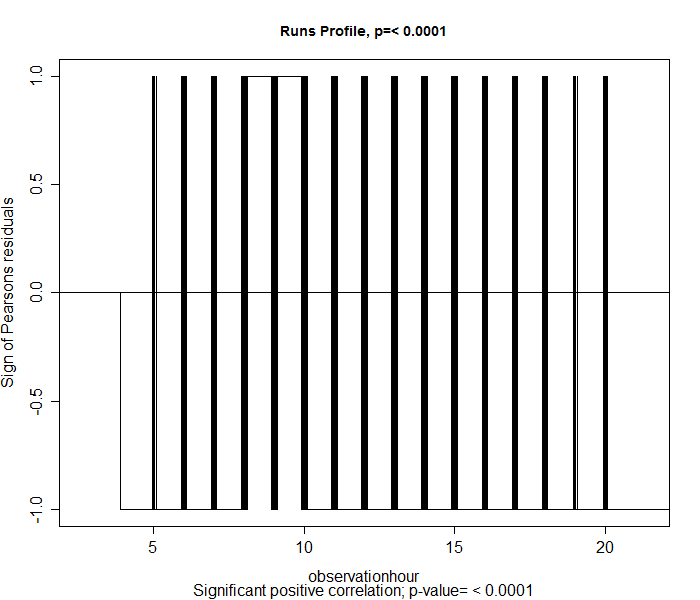
\includegraphics[width=6cm]{bc/RunsProfile_observationhour_glmk1.png}
\label{fig:sub:runs1a}
}	
  \hfill
  \subfloat[]{
        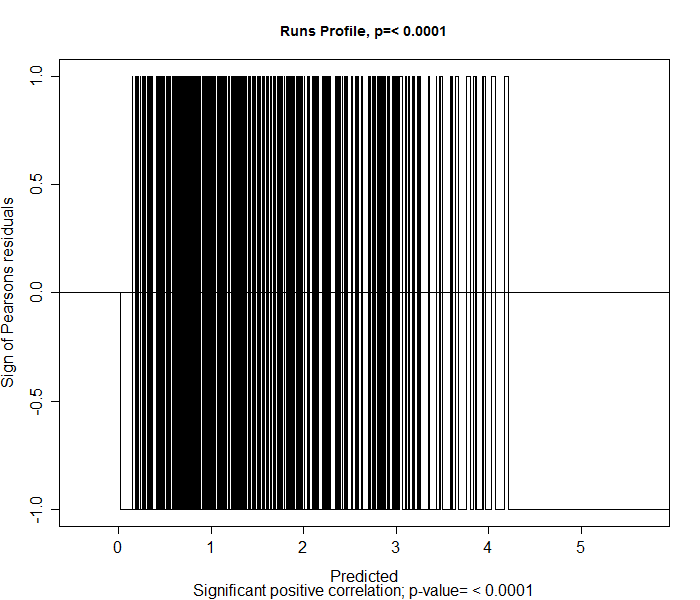
\includegraphics[width=6cm]{bc/RunsProfile_Predicted_glmk1.png}
\label{fig:sub:runs1b}
}	
  \hfill
   \subfloat[]{
      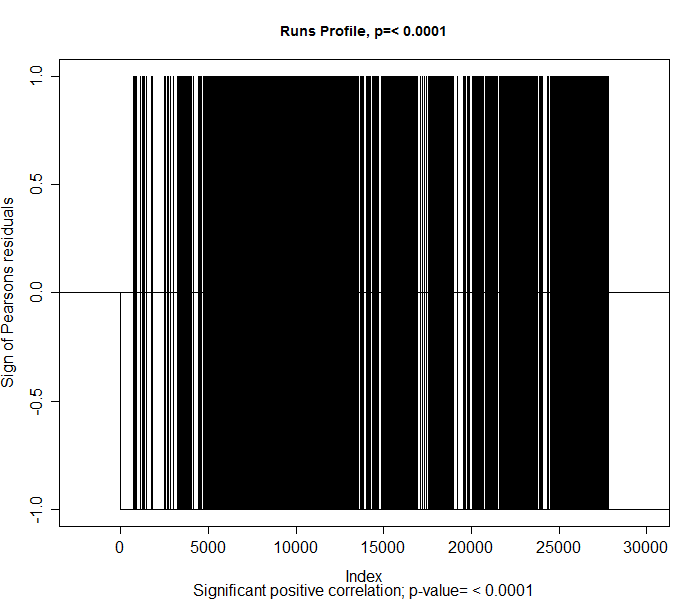
\includegraphics[width=6cm]{bc/RunsProfile_Index_glmk1.png}
\label{fig:sub:runs1c}
}	
  \hfill
\caption{Runs profiles for residuals ordered by (a) observation hour, (b) predicted value and (c) temporally (by observation index). The $p$-values and text presented on each plot indicate if there is correlation present in the residuals.  The lines are the strings of sequences of positive and negative residuals.  A vertical line is the switch between a positive and negative run (or vice versa).}
\label{fig:nsruns1}
\end{figure}
\end{frame}

\begin{frame}
\begin{itemize}
\item Runs test and plots show an issue with correlated residuals
\item We have positive correlation in the residuals no matter how they are ordered
%\item Observation hour could be modelled appropriately according to the cumulative residual plot.  However, the black line may mask the expected line in places.
\bigskip
\item Conclusion:  
\begin{itemize}
  \item We have correlation that must be accounted for
  %\item we might want to consider more flexibility for {\tt observationhour}.
\end{itemize}
\end{itemize}
\end{frame}

\begin{frame}
\frametitle{Choosing a blocking structure to model correlation.}
\begin{itemize}
\item Correlation within blocks should decline to approximately zero 
\item Between blocks residuals should be independent
\item Blocks are usually determined by looking at the sampling design
\item Here we use the unique cell identifier within each day of observation: Each grid cell is considered independent but residuals may be non-independent within a block.
\item There are 41 grid cells repeated several days a month, for 12 months over four years times, giving us 5576 blocks.
\end{itemize}
\end{frame}


\begin{frame}[fragile]
\frametitle{Autocorrelation function plot}
We can check the correlation declines within our blocks by plotting the autocorrelation of the model residuals by block (Figure \ref{fig:nsacf}).  First make a column in the data (if it does not already exist) that represents the blocking structure.

\begin{knitrout}\footnotesize
\definecolor{shadecolor}{rgb}{0.969, 0.969, 0.969}\color{fgcolor}\begin{kframe}
\begin{alltt}
data$blockid <- \hlfunctioncall{paste}(data$GridCode, data$Year, data$MonthOfYear, 
    data$DayOfMonth, sep = \hlstring{""})
\hlcomment{# **** blockid must be a factor or numeric, not a character ****}
data$blockid <- \hlfunctioncall{as.factor}(data$blockid)
 \hlfunctioncall{runACF}(data$blockid, fullModel, store = F)
\end{alltt}
\end{kframe}
\end{knitrout}


\begin{itemize}
\item Some blocks have little correlation, whilst others have high correlation (0.5) at a lag of 6 (data points are at hourly intervals so a lag of 6 is 6 hours.)
\item It is these blocks with the higher correlation that must be accounted for
\item Conclusion: Our blocking structure is suitable
\end{itemize}
\end{frame}

\begin{frame}[fragile]
\begin{figure}[h!]
  \centering
  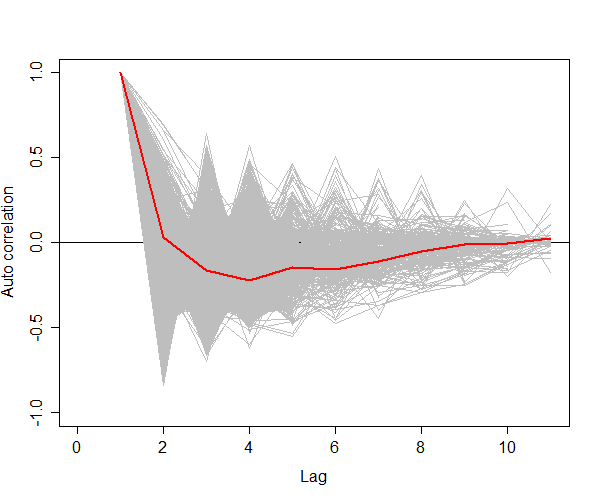
\includegraphics[width=9cm]{bc/acfPlot.png}
\caption{Plot of the correlation in residuals for each block (grey lines).  The mean correlation at each lag is indicated in red.}
\label{fig:nsacf}
\end{figure}
\end{frame}



%~~~~~~~~~~~~~~~~~~~~~~~~~~~~~~~~~~~~~~~~~
%~~~~~~~~~~~~~~~~~~~~~~~~~~~~~~~~~~~~~~~~~~~

\subsection{Model Selection}
\begin{frame}[fragile]
Select what one-dimensional covariates to include in the model and use SALSA to determine the knot locations of those that are continuous: {\tt observation hour}.

\noindent We can use cumulative residual plots to check for \textbf{appropriately modelled covariates}.  
\begin{itemize}
\item Cumulative residuals are sequentially summed raw residuals on the scale of the response.
\item These plots show systematic over- or under- prediction.  
\item We expect to see good mixing (lots of peaks and troughs) and deviation from this may indicate the covariate is not modelled appropriately.
\item Figure \ref{fig:nscumres1} shows cumulative residual plots from a model with depth modelled as a linear term and with one knot at the mean.
\end{itemize} 
\end{frame}

\begin{frame}[fragile]
\frametitle{Plotting Cumulative Residuals}
\begin{knitrout}\footnotesize
\definecolor{shadecolor}{rgb}{0.969, 0.969, 0.969}\color{fgcolor}\begin{kframe}
\begin{alltt}
\hlcomment{# plot cumulative residuals for model with observationhour as smooth term}
\hlfunctioncall{plotCumRes}(fullModel, varlist= \hlfunctioncall{c}(\hlstring{"observationhour"}), splineParams)
\end{alltt}
\begin{verbatim}
"Calculating cumulative residuals"
\end{verbatim}
\end{kframe}
\end{knitrout}

\begin{figure}[h]
  \centering
 \subfloat[]{
  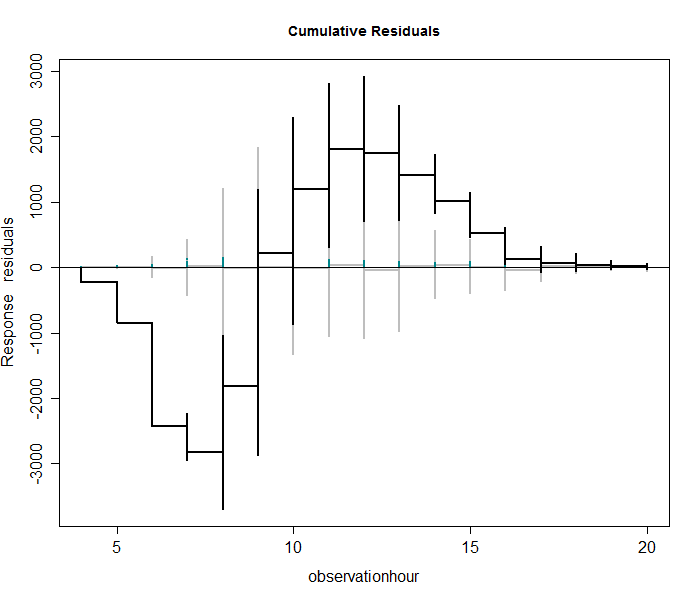
\includegraphics[width=6cm]{bc/CumRes_observationhour_glm.png}
\label{fig:sub:nscumres1a}
}	
  \hfill
  \subfloat[]{
        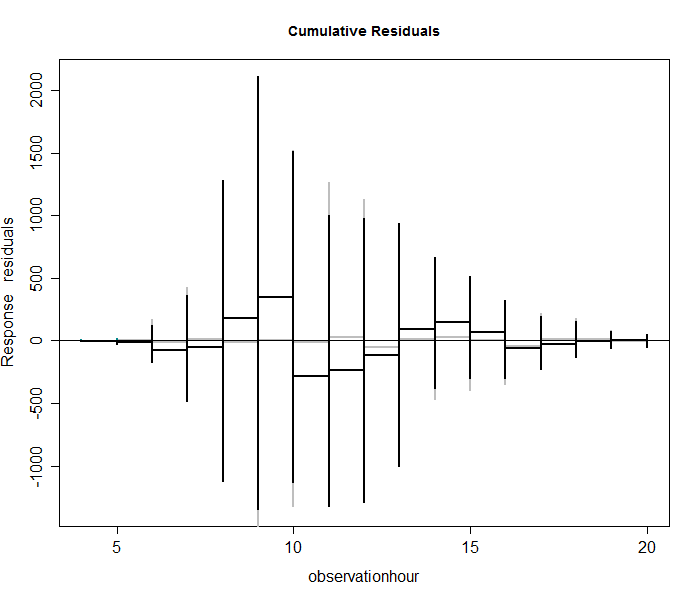
\includegraphics[width=6cm]{bc/CumRes_observationhour_glmk1.png}
\label{fig:sub:nscumres1b}
}	
\caption{Cumulative residual plots residuals ordered by observation hour. (a) observation hour modelled as a linear term and (b) depth modelled with one knot at the mean observation hour.  The blue points are the residual values, the black line represents the cumulative residuals. The grey line in the background is what we would expect the cumulative residuals to be if observation hour was modelled correctly.}
\label{fig:nscumres1}
\end{figure}
\end{frame}

\begin{frame}
\frametitle{Cumulative Residuals}
\begin{itemize}
\item Observation hour as a linear term is not appropriate (Figure \ref{fig:sub:nscumres1a}).
\item The black line (our model) does not correspond well with the expected line (grey) and shows systematic over prediction at early hours and under prediction in the early afternoon.
\item Observation hour as a smooth term with one knot at the mean is much better but the black line may mask the expected line in places due to the discrete nature of the variable (Figure \ref{fig:sub:nscumres1b}).
\pause
\item Conclusion:  
\begin{itemize}
  \item we might want to consider more flexibility for {\tt observationhour} by using SALSA.
\end{itemize}
\end{itemize}
\end{frame}


\begin{frame}[fragile]
\frametitle{Setting up the model for SALSA}
\begin{itemize}
\item There must be a column called {\tt response} in the data, which is the response variable used in the initial model to be fitted.
\item The argument {\tt salsa1dlist} contains parameters for the {\tt runSALSA1D} function.  
\begin{itemize}
\item {\tt fitnessMeasure}. The criterion for selecting the `best' model.  Available options: AIC, AIC$_c$, BIC, QIC$_b$.
\item {\tt minKnots\_1d}. Minimum number of knots to be tried.
\item {\tt maxKnots\_1d}. Maximum number of knots to be tried.
\item {\tt startKnots\_1d}. Starting number of knots (spaced at quantiles of the data).
\item {\tt degree}. The degree of the B-spline. Does not need to be specified if {\tt splineParams} is a parameter in {\tt runSALSA1D}.
\item {\tt maxIterations}. The exchange/improve steps will terminate after maxIterations if still running.
\item {\tt gaps}. The minimum gap between knots (in unit of measurement of explanatory).
\end{itemize}
\item The initial model contains all the factor level covariates and any covariates of interest that are not specified in the {\tt varlist} argument of {\tt runSALSA1D}.
\end{itemize}


\begin{knitrout}\footnotesize
\definecolor{shadecolor}{rgb}{0.969, 0.969, 0.969}\color{fgcolor}\begin{kframe}
\begin{alltt}
\hlcomment{#info for SALSA}
data$response <- data$birds

\hlcomment{# set initial model without the spline terms}
initialModel <- \hlfunctioncall{glm}(response ~ \hlfunctioncall{as.factor}(floodebb) + \hlfunctioncall{as.factor}(impact) + 
    \hlfunctioncall{offset}(\hlfunctioncall{log}(area)), family = \hlstring{"quasipoisson"}, data = data)


salsa1dlist <- \hlfunctioncall{list}(fitnessMeasure = \hlstring{"QICb"}, minKnots_1d = 2, 
    maxKnots_1d = 20, startKnots_1d = 2, degree = 2, maxIterations = 10, 
    gaps = \hlfunctioncall{c}(1))

\end{alltt}
\end{kframe}
\end{knitrout}

\begin{knitrout}\footnotesize
\definecolor{shadecolor}{rgb}{0.969, 0.969, 0.969}\color{fgcolor}\begin{kframe}
\begin{alltt}
\hlcomment{# run SALSA}
salsa1dOutput <- \hlfunctioncall{runSALSA1D}(initialModel, salsa1dlist, varlist=
    \hlfunctioncall{c}(\hlstring{"observationhour"}), factorlist=\hlfunctioncall{c}(\hlstring{"floodebb"}, \hlstring{"impact"}), predictData, 
    splineParams=splineParams)
\end{alltt}
\end{kframe}
\end{knitrout}

\end{frame}

\begin{frame}[fragile]
\noindent Let's look at the structure of the output: 
\begin{itemize}
\item {\tt bestModel}. The model object for the best fitted model.
\item {\tt modelFits1D}.  Each slot in the list shows the term fitted, the fit statistic resulting from that term, the knots used and finally the overall formula.  If {\tt varlist} is more than one covariate, this output shows how each covariate was retained and what knots were finalised.
\item {\tt splineParams}.  The spline parameter object is updated with the new knot numbers and locations of the covariates from {\tt varlist}.
\item {\tt fitStat}.  The fit statistic of the best model.
\end{itemize}

\begin{knitrout}\footnotesize
\definecolor{shadecolor}{rgb}{0.969, 0.969, 0.969}\color{fgcolor}\begin{kframe}
\begin{alltt}
\hlfunctioncall{str}(salsa1dOutput, max.level = 1)
\end{alltt}
\begin{verbatim}
List of 4
 $ bestModel   :List of 30
  ..- attr(*, "class")= chr [1:2] "glm" "lm"
 $ modelFits1D :List of 2
 $ splineParams:List of 2
 $ fitStat     : num 34341
\end{verbatim}
\end{kframe}
\end{knitrout}
\end{frame}

\begin{frame}[fragile]
\begin{knitrout}\footnotesize
\definecolor{shadecolor}{rgb}{0.969, 0.969, 0.969}\color{fgcolor}\begin{kframe}
\begin{alltt}
\hlcomment{# knots chosen for observation hour}
salsa1dOutput$splineParams[[2]]$knots
\end{alltt}
\begin{verbatim}
[1]  9 15 17
\end{verbatim}
\end{kframe}
\end{knitrout}

\begin{itemize}
\item Initial model - one knot at the mean observation hour (12pm) 
\item SALSA result - three knots selected (see output above)
\item The result of SALSA is additional flexibility added to the model for the relationship between bird counts and observation hour.
\end{itemize}
\end{frame}

\begin{frame}[fragile]
\frametitle{Spatial component}
\begin{itemize}
\item Next we add a two dimensional smooth of geographic coordinates (s({\tt x.pos}, {\tt y.pos}))
\item To test for a redistribution of animals with an impact effect we fit an interaction term between the smooth of coordinates and {\tt impact}.
\item SALSA is used to determine spatially adaptive knot locations for this smooth term.
\end{itemize}
\end{frame}

\begin{frame}
\begin{block}{SALSA 2D requirements}
\begin{itemize}
\item A grid of knot locations
\item Matrix of knot to knot distances 
\item Matrix of data to knot distances
\item Vector of range parameters for CReSS (determines the range of effectiveness of each knot basis).  See \citep{ScottH2013} for more details.
\item Minimum, maximum and starting number of knots
\end{itemize}
\end{block}
\noindent The next section assumes that the knot grid has been defined. See section \ref{tips:subsec:salsa} for some guidance to do this.
\end{frame}

\begin{frame}[fragile]
\frametitle{Spatial component}
\begin{knitrout}\footnotesize
\definecolor{shadecolor}{rgb}{0.969, 0.969, 0.969}\color{fgcolor}\begin{kframe}
\begin{alltt}
\hlcomment{# load knotgrid (regular grid containing NA's for invalid knot }
\hlcomment{# locations (e.g. on land or outside study region))}
\hlfunctioncall{data}(knotgrid.ns)
knotgrid <- knotgrid.ns
\end{alltt}
\end{kframe}
\end{knitrout}

\noindent The knot points in {\tt knotgrid} are located at the centre of each of the grid cells containing data.
\end{frame}

\begin{frame}[fragile]
\noindent The distance matrices give the distance between the data and the knots in one matrix and the second matrix is the knot to knot distances.  The function {\tt makeDists} calculates Euclidean distance, however, the {\tt runSALSA2D} function may also take geodesic distance matrices (as the fish swims rather than as the crow flies).  See \citet{ScottH2013} for more details on geodesic distances.

\begin{knitrout}\footnotesize
\definecolor{shadecolor}{rgb}{0.969, 0.969, 0.969}\color{fgcolor}\begin{kframe}
\begin{alltt}
\hlcomment{# make distance matrices for datatoknots and knottoknots}
distMats <- \hlfunctioncall{makeDists}(\hlfunctioncall{cbind}(data$x.pos, data$y.pos), \hlfunctioncall{na.omit}(knotgrid))
\hlfunctioncall{str}(distMats)
\end{alltt}
\begin{verbatim}
List of 2
 $ dataDist: num [1:27798, 1:41] 4000 4000 4000 4000 4000 4000 4000 ...
 $ knotDist: num [1:41, 1:41] 0 1000 2000 3000 4000 ...
  ..- attr(*, "dimnames")=List of 2
  .. ..$ : chr [1:41] "3" "4" "5" "6" ...
  .. ..$ : chr [1:41] "3" "4" "5" "6" ...
\end{verbatim}
\end{kframe}
\end{knitrout}

\noindent A sequence of range parameters is required for the CReSS smooth.  
\begin{itemize}
\item The range parameter determines the influence of each selected knot.  
\item Small numbers are for a local influence and large ones a global influence.
\item Once knot locations are selected (using the mid value in the range sequence), SALSA selects the appropriate range parameter (from the sequence created below) for each knot.
\item {\tt getRadiiChoices} selects a number of radii (default = 8) based on the distances in the data to knot distance matrix created above.
\end{itemize}
\begin{knitrout}\footnotesize
\definecolor{shadecolor}{rgb}{0.969, 0.969, 0.969}\color{fgcolor}\begin{kframe}
\begin{alltt}
\hlcomment{# create sequence of radii}
r_seq <- \hlfunctioncall{getRadiiChoices}(numberofradii=8, distMats$dataDist)
\end{alltt}
\end{kframe}
\end{knitrout}
\end{frame}

\begin{frame}[fragile]
\frametitle{Setting up the spatial SALSA components}

\begin{itemize}
\item {\tt fitnessMeasure}. The fitness measures available are the same as for {\tt runSALSA1D}.
\item {\tt knotgrid}. $(k \times 2)$ matrix of knot coordinates.  Rows of {\tt NA}'s identify illegal knot locations
\item {\tt startKnots}. Number of space-filled knots to start with (between minKnots and maxKnots)
\item {\tt minKnots}.  Minimum number of knots to fit
\item {\tt maxKnots}.  Maximum number of knots to fit
\item {\tt r\_seq}. Sequence of range parameters for the CReSS basis.
\item {\tt gap}.  Minimum gap between knots (in unit of measurement of {\tt x.pos} and {\tt y.pos})
\item {\tt interactionTerm}. Specifies which term in the model the spatial smooth will interact with. If NULL no interaction term is fitted.
\end{itemize}

\begin{knitrout}\footnotesize
\definecolor{shadecolor}{rgb}{0.969, 0.969, 0.969}\color{fgcolor}\begin{kframe}
\begin{alltt}
\hlcomment{# make parameter set for running salsa2d}
salsa2dlist <- \hlfunctioncall{list}(fitnessMeasure = \hlstring{"QICb"}, knotgrid = knotgrid, 
    startKnots = 6, minKnots = 4, maxKnots = 20, r_seq = r_seq, 
    gap = 1, interactionTerm = \hlstring{"\hlfunctioncall{as.factor}(impact)"})
\end{alltt}
\end{kframe}
\end{knitrout}

\noindent The initial model is the best model from the one-dimensional SALSA results.
\begin{knitrout}\footnotesize
\definecolor{shadecolor}{rgb}{0.969, 0.969, 0.969}\color{fgcolor}\begin{kframe}
\begin{alltt}
\hlcomment{# splineParams must be an object in workspace}
\hlcomment{# update splineParams with the SALSA1D results}
splineParams <- salsa1dOutput$splineParams
salsa2dOutput_k6 <- \hlfunctioncall{runSALSA2D}(salsa1dOutput$bestModel, salsa2dlist, 
    distMats$dataDist, distMats$knotDist, splineParams = splineParams)
\end{alltt}
\end{kframe}
\end{knitrout}
\end{frame}

\begin{frame}[fragile]
\frametitle{Multiple SALSA runs}

\noindent The example above uses 6 starting knot locations.  There is a risk that the SALSA algorithm may get stuck in local minima or maxima and so we recommend that a variety of starting knot numbers are used.  Here we try 6, 8, 10, 12, 14 and 16 (Table \ref{tab:nsfitstats}).  \\

\noindent We use $k$-fold Cross-Validation (CV) as a method for selecting between models with a variety of starting knots.\\

Example:
\begin{knitrout}\footnotesize
\definecolor{shadecolor}{rgb}{0.969, 0.969, 0.969}\color{fgcolor}\begin{kframe}
\begin{alltt}
data$foldid <- \hlfunctioncall{getCVids}(data, folds = 5, block = \hlstring{"blockid"})
\end{alltt}
\end{kframe}
\end{knitrout}


\begin{knitrout}\footnotesize
\definecolor{shadecolor}{rgb}{0.969, 0.969, 0.969}\color{fgcolor}\begin{kframe}
\begin{alltt}
cv1 <- \hlfunctioncall{getCV_CReSS}(salsa1dOutput$bestModel, salsa1dOutput$splineParams)
\end{alltt}
\begin{verbatim}
[1] 33.91
\end{verbatim}
\end{kframe}
\end{knitrout}

\end{frame}

\begin{frame}[fragile]
\frametitle{Choosing a model}
\begin{table}[h]
\caption{Table of CV scores for a variety of starting knot numbers for the spatial smooth.}
\centering
\begin{tabular}{l|c|c|c}
\textbf{Model type} & \textbf{Start knots} & \textbf{End knots}  & \textbf{CV}\\
\hline
1D terms only & - & - & 33.9058\\
1D/2D terms & 6 & 6  & 28.6426\\
1D/2D terms & 8 & 8  & 28.1481\\
1D/2D terms & 10 & 10  & 27.9571\\
1D/2D terms & 12 & 12  & 27.0373\\
1D/2D terms & 14 & 14  & 27.0474\\
1D/2D terms & 16 & 16  & 27.0367\\
\end{tabular}
\label{tab:nsfitstats}
\end{table}
\end{frame}


\begin{frame}[fragile]
\noindent The best model chosen using CV score is the model that uses a spatial smooth with 16 spatial knots.
\begin{knitrout}\footnotesize
\definecolor{shadecolor}{rgb}{0.969, 0.969, 0.969}\color{fgcolor}\begin{kframe}
\begin{alltt}
\hlcomment{# having chosen the 2d interaction model, save the model object}
baseModel <- salsa2dOutput_k16$bestModel
\hlcomment{# update spline parameter object}
splineParams <- salsa2dOutput_k16$splineParams
\end{alltt}
\end{kframe}
\end{knitrout}

\end{frame}

%~~~~~~~~~~~~~~~~~~~~~~~~~~~~~~~~~~~~~~~~~
%~~~~~~~~~~~~~~~~~~~~~~~~~~~~~~~~~~~~~~~~~~~

\subsection{Checking $p$-values}

\begin{frame}[fragile]
\frametitle{Re-assessing runs test for best model}
\begin{itemize}
\item Our `best' model based on CV selection is the model with the interaction term. 
\item We could also use $p$-value selection, though the model must be fitted as a GEE to model the correlation.
\end{itemize}

We must account for the correlation in our residuals, which was found earlier, but should also check the current model.
\begin{knitrout}\footnotesize
\definecolor{shadecolor}{rgb}{0.969, 0.969, 0.969}\color{fgcolor}\begin{kframe}
\begin{alltt}
\hlfunctioncall{runs.test}(\hlfunctioncall{residuals}(baseModel, type = \hlstring{"pearson"}))
\end{alltt}
\begin{verbatim}
	Runs Test - Two sided
data:  residuals(baseModel, type = "pearson") 
Standardized Runs Statistic = -88.67, p-value < 2.2e-16
\end{verbatim}
\end{kframe}
\end{knitrout}
\end{frame}


\begin{frame}[fragile]
\frametitle{GEE framework}
\noindent There is significant positive residual correlation ($p<<0.05$ and test statistic is negative) so we re-fit the model as a GEE.\\

\noindent Note: It is possible to do this at this stage as we are modelling correlation using empirical standard errors and not a specific correlation structure.

\bigskip
\noindent The current model:
\footnotesize
\begin{verbatim}
glm(formula = response ~ as.factor(floodebb) + as.factor(impact) + 
    bs(observationhour, knots = splineParams[[2]]$knots, degree = 
    splineParams[[2]]$degree, Boundary.knots = splineParams[[2]]$bd) + 
    LocalRadialFunction(radiusIndices, dists, radii, aR) + 
    as.factor(impact):LocalRadialFunction(radiusIndices, dists, radii, aR) + 
    offset(log(area)), family = quasipoisson, data = data)
\end{verbatim}
\normalsize
\end{frame}

\begin{frame}[fragile]
\begin{knitrout}\footnotesize
\definecolor{shadecolor}{rgb}{0.969, 0.969, 0.969}\color{fgcolor}\begin{kframe}
\begin{alltt}
\hlcomment{# N.B. for the GEE formula, the data must be ordered by block (which this is)}
\hlcomment{# and the blockid must be numeric}
\hlcomment{# specify parameters for local radial:}
radiusIndices <- splineParams[[1]]$radiusIndices
dists <- splineParams[[1]]$dist
radii <- splineParams[[1]]$radii
aR <- splineParams[[1]]$invInd[splineParams[[1]]$knotPos]

\hlcomment{# update model in workspace with parameters for spatial smooth (above)}
baseModel <- \hlfunctioncall{update}(baseModel, . ~ .)
\end{alltt}
\end{kframe}
\end{knitrout}

\noindent The {\tt baseModel} is updated with the parameters returned by SALSA2D using the {\tt update} function\footnote{The update function is part of the basic functionality in {\tt R} and can be used to quickly re-fit a model removing or adding covariates, changing the family or data set or in this case refreshing the parameters used in {\tt LocalRadialFunction}.}.  This makes sure that the {\tt baseModel} object is made using the parameters currently in the workspace.

\begin{knitrout}\footnotesize
\definecolor{shadecolor}{rgb}{0.969, 0.969, 0.969}\color{fgcolor}\begin{kframe}
\begin{alltt}

\hlcomment{# Re-fit the chosen model as a GEE (based on SALSA knot placement) and}
\hlcomment{# GEE p-values}
geeModel <- \hlfunctioncall{geeglm}(\hlfunctioncall{formula}(baseModel), data = data, family = poisson,
                   id = blockid)
\end{alltt}
\end{kframe}
\end{knitrout}
\noindent Note:  The family specified for the GEE model is Poisson because the dispersion parameter is automatically estimated using {\tt geeglm}. Therefore, we need not (and cannot) specify the quasi-Poisson family.
\end{frame}

\begin{frame}[fragile]
\frametitle{Checking $p$-values}
\begin{knitrout}\footnotesize
\definecolor{shadecolor}{rgb}{0.969, 0.969, 0.969}\color{fgcolor}\begin{kframe}
\begin{alltt}
\hlcomment{# table of p-values (specifying varlist and factorlist}
\hlcomment{# makes shorter variable names)}
\hlfunctioncall{getPvalues}(geeModel, varlist = \hlfunctioncall{c}(\hlstring{"observationhour"}), factorlist = \hlfunctioncall{c}(\hlstring{"floodebb"}, 
    \hlstring{"impact"}))
\end{alltt}
\begin{verbatim}
[1] "Getting marginal p-values"
                Variable  p-value
1               floodebb  <0.0001
2                 impact   0.5615
3        observationhour  <0.0001
4        s(x.pos, y.pos)  <0.0001
5 s(x.pos, y.pos):impact   0.0241
\end{verbatim}
\end{kframe}
\end{knitrout}

\end{frame}


\begin{frame}[fragile]
\frametitle{Do we remove the main {\tt impact} effect?}
\begin{itemize}
\item Keep the main effect for {\tt impact} because it is part of the interaction term and is difficult to interpret.\\
\item Fit a model without the interaction term to test for a significant increase/decrease pre and post impact.\\
\item If the interaction is significant but the {\tt impact} term in a model without the interaction is not significant then there has been a re-distribution of animals but no overall change.\\
\item This is the case for this model.  $p$>>0.05 for {\tt impact} in a model with no interaction term.\\
\end{itemize}

\bigskip
Below is an example of how to remove the interaction term using the {\tt update} function.
\end{frame}

\begin{frame}[fragile]
\frametitle{Removing the main {\tt impact} effect}
\begin{knitrout}\footnotesize
\definecolor{shadecolor}{rgb}{0.969, 0.969, 0.969}\color{fgcolor}\begin{kframe}
\begin{alltt}
\hlcomment{# how to remove impact}
noint.model<-\hlfunctioncall{update}(geeModel, .~. - \hlfunctioncall{as.factor}(impact):
                     \hlfunctioncall{LocalRadialFunction}(radiusIndices, dists, radii, aR))
\hlcomment{# reshow p-values}
\hlfunctioncall{getPvalues}(noint.model, varlist = \hlfunctioncall{c}(\hlstring{"observationhour"}), factorlist = \hlfunctioncall{c}(\hlstring{"floodebb"}, 
    \hlstring{"impact"}))
\end{alltt}
\begin{verbatim}

[1] "Getting marginal p-values"
                Variable  p-value
1               floodebb  <0.0001
2                 impact   0.5615
3        observationhour  <0.0001
4        s(x.pos, y.pos)  <0.0001
\end{verbatim}
\end{kframe}
\end{knitrout}

\end{frame}


%~~~~~~~~~~~~~~~~~~~~~~~~~~~~~~
%~~~~~~~~~~~~~~~~~~~~~~~~~~~~~~~~~
\subsection{Assessing covariate relationships}

\begin{frame}[fragile]
\begin{block}{Partial Residual Plots\footnote{see `component-plus-residual' plots in \citet{Fox2011} for more details.}}
These plots allow visual examination the one-dimensional covariates in the model (observation hour, tide state and impact) and to check that smooth/linear terms are specified correctly.\\

\noindent The partial residuals, $e_{ij}$,  for predictor $x_j$ are formed by adding the fitted linear component in this predictor to the least squares residuals\footnote{$e_{ij} = e_i + b_jx_{ij}$}.  The partial residuals are then plotted against $x_j$
\end{block}

\begin{knitrout}\footnotesize
\definecolor{shadecolor}{rgb}{0.969, 0.969, 0.969}\color{fgcolor}\begin{kframe}
\begin{alltt}
\hlfunctioncall{runPartialPlots}(geeModel, data, factorlist = \hlfunctioncall{c}(\hlstring{"floodebb"}, \hlstring{"impact"}), 
    varlist = \hlfunctioncall{c}(\hlstring{"observationhour"}))
\end{alltt}
\begin{verbatim}
[1] "Making partial plots"
\end{verbatim}
\end{kframe}
\end{knitrout}

\end{frame}

\begin{frame}[fragile]
\frametitle{Assessing covariate relationships}
\begin{figure}[h!]
  \centering
  \subfloat[]{
    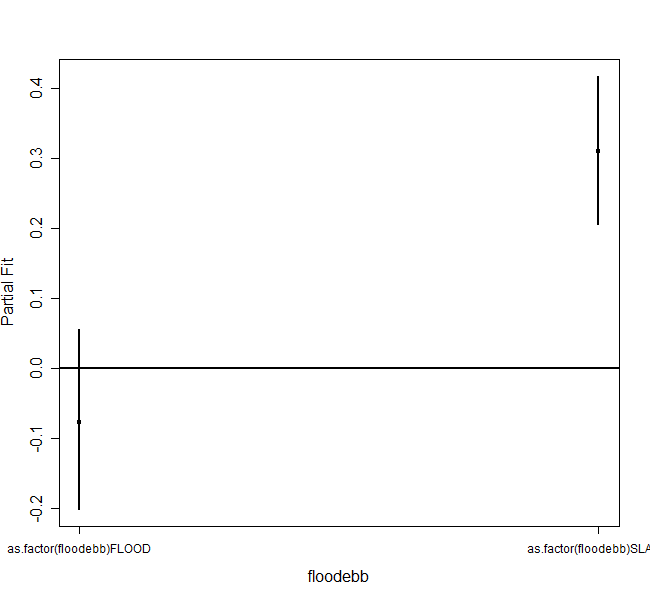
\includegraphics[width=6cm]{bc/PartialFits1.png}
  }
  \subfloat[]{
    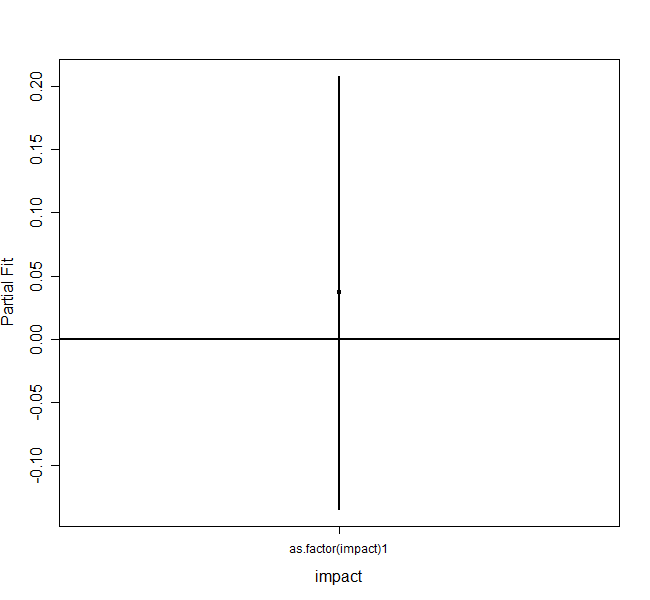
\includegraphics[width=6cm]{bc/PartialFits2.png}
  }
  \hfill
  \subfloat[]{
    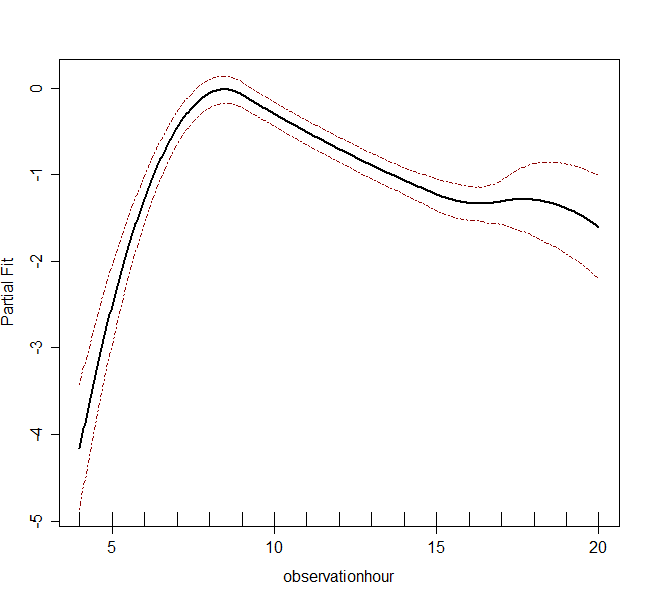
\includegraphics[width=6cm]{bc/PartialFits3.png}
  }
  \caption{Partial plots for (a) tide state, (b) impact and (c) observation hour.}
  \label{fig:partials}
\end{figure}
\end{frame}

\begin{frame}
\frametitle{Partial Plots}
\begin{itemize}
\item Tide state: predictions for flood are not significantly different to ebb (baseline)
\item There are, on average, more animals seen during slack tide than for the baseline (ebb). \pause
\item Impact: confirms the ANOVA $p$-value (seen earlier; $p>>0.05$) and indicates no change in bird numbers post impact.
\pause
\item Observation hour: a peaked non-linear relationship with maximum birds seen between 8 and 11am.
\item Small confidence interval indicates a precisely estimated relationship.
\end{itemize}
\pause
\bigskip
Note: if the confidence interval for observation hour was very wide it might indicate that observation hour as a linear term is more appropriate.
\end{frame}

\clearpage
%~~~~~~~~~~~~~~~~~~~~~~~~~~~~~~~~~~~~~~~~~
%~~~~~~~~~~~~~~~~~~~~~~~~~~~~~~~~~~~~~~~~~~~

\section{Diagnostics}

\begin{frame}[fragile]
\frametitle{Diagnostics}
We make multiple plots to assess the fit of our model:

\bigskip
\begin{itemize}
\item Observed vs Fitted
\item Fitted vs residuals
\item Cumulative residuals
\item Runs sequence
\item COVRATIO statistics
\item PRESS statistics
\item Raw residuals
\end{itemize}
\end{frame}

\begin{frame}[fragile]
\frametitle{Observed vs fitted Plot}

\begin{block}{Observed vs Fitted}
Indication of fit to the data.  All the values would be on the 45$^o$ line for a perfectly fitting model.    
\end{block}

The agreement between the input data and the model undergoing evaluation can be quantified using numerical measures; Marginal R-squared and Concordance Correlation. 
\end{frame}

\begin{frame}[fragile]
These measure are output on the observed vs fitted plot created using the {\tt runDiagnostics} function. 

\begin{block}{Marginal R-squared value}
It is widely used to assess models fitted to both un-correlated and correlated data and is approximately between 0 and 1.  Values closer to 1 indicate better fit to the data.
\end{block}

\begin{block}{Concordance Correlation}
It is guaranteed to return values between zero and one.  Values closer to 1 indicate better fit to the data.
\end{block}

\begin{knitrout}\footnotesize
\definecolor{shadecolor}{rgb}{0.969, 0.969, 0.969}\color{fgcolor}\begin{kframe}
\begin{alltt}
\hlcomment{# create observed vs fitted and fitted vs residual plots}
\hlfunctioncall{runDiagnostics}(geeModel)
\end{alltt}
\begin{verbatim}
[1] "Assessing predictive power"
\end{verbatim}
\end{kframe}
\end{knitrout}

\end{frame}

\begin{frame}[fragile]
\begin{figure}[h]
  \centering
    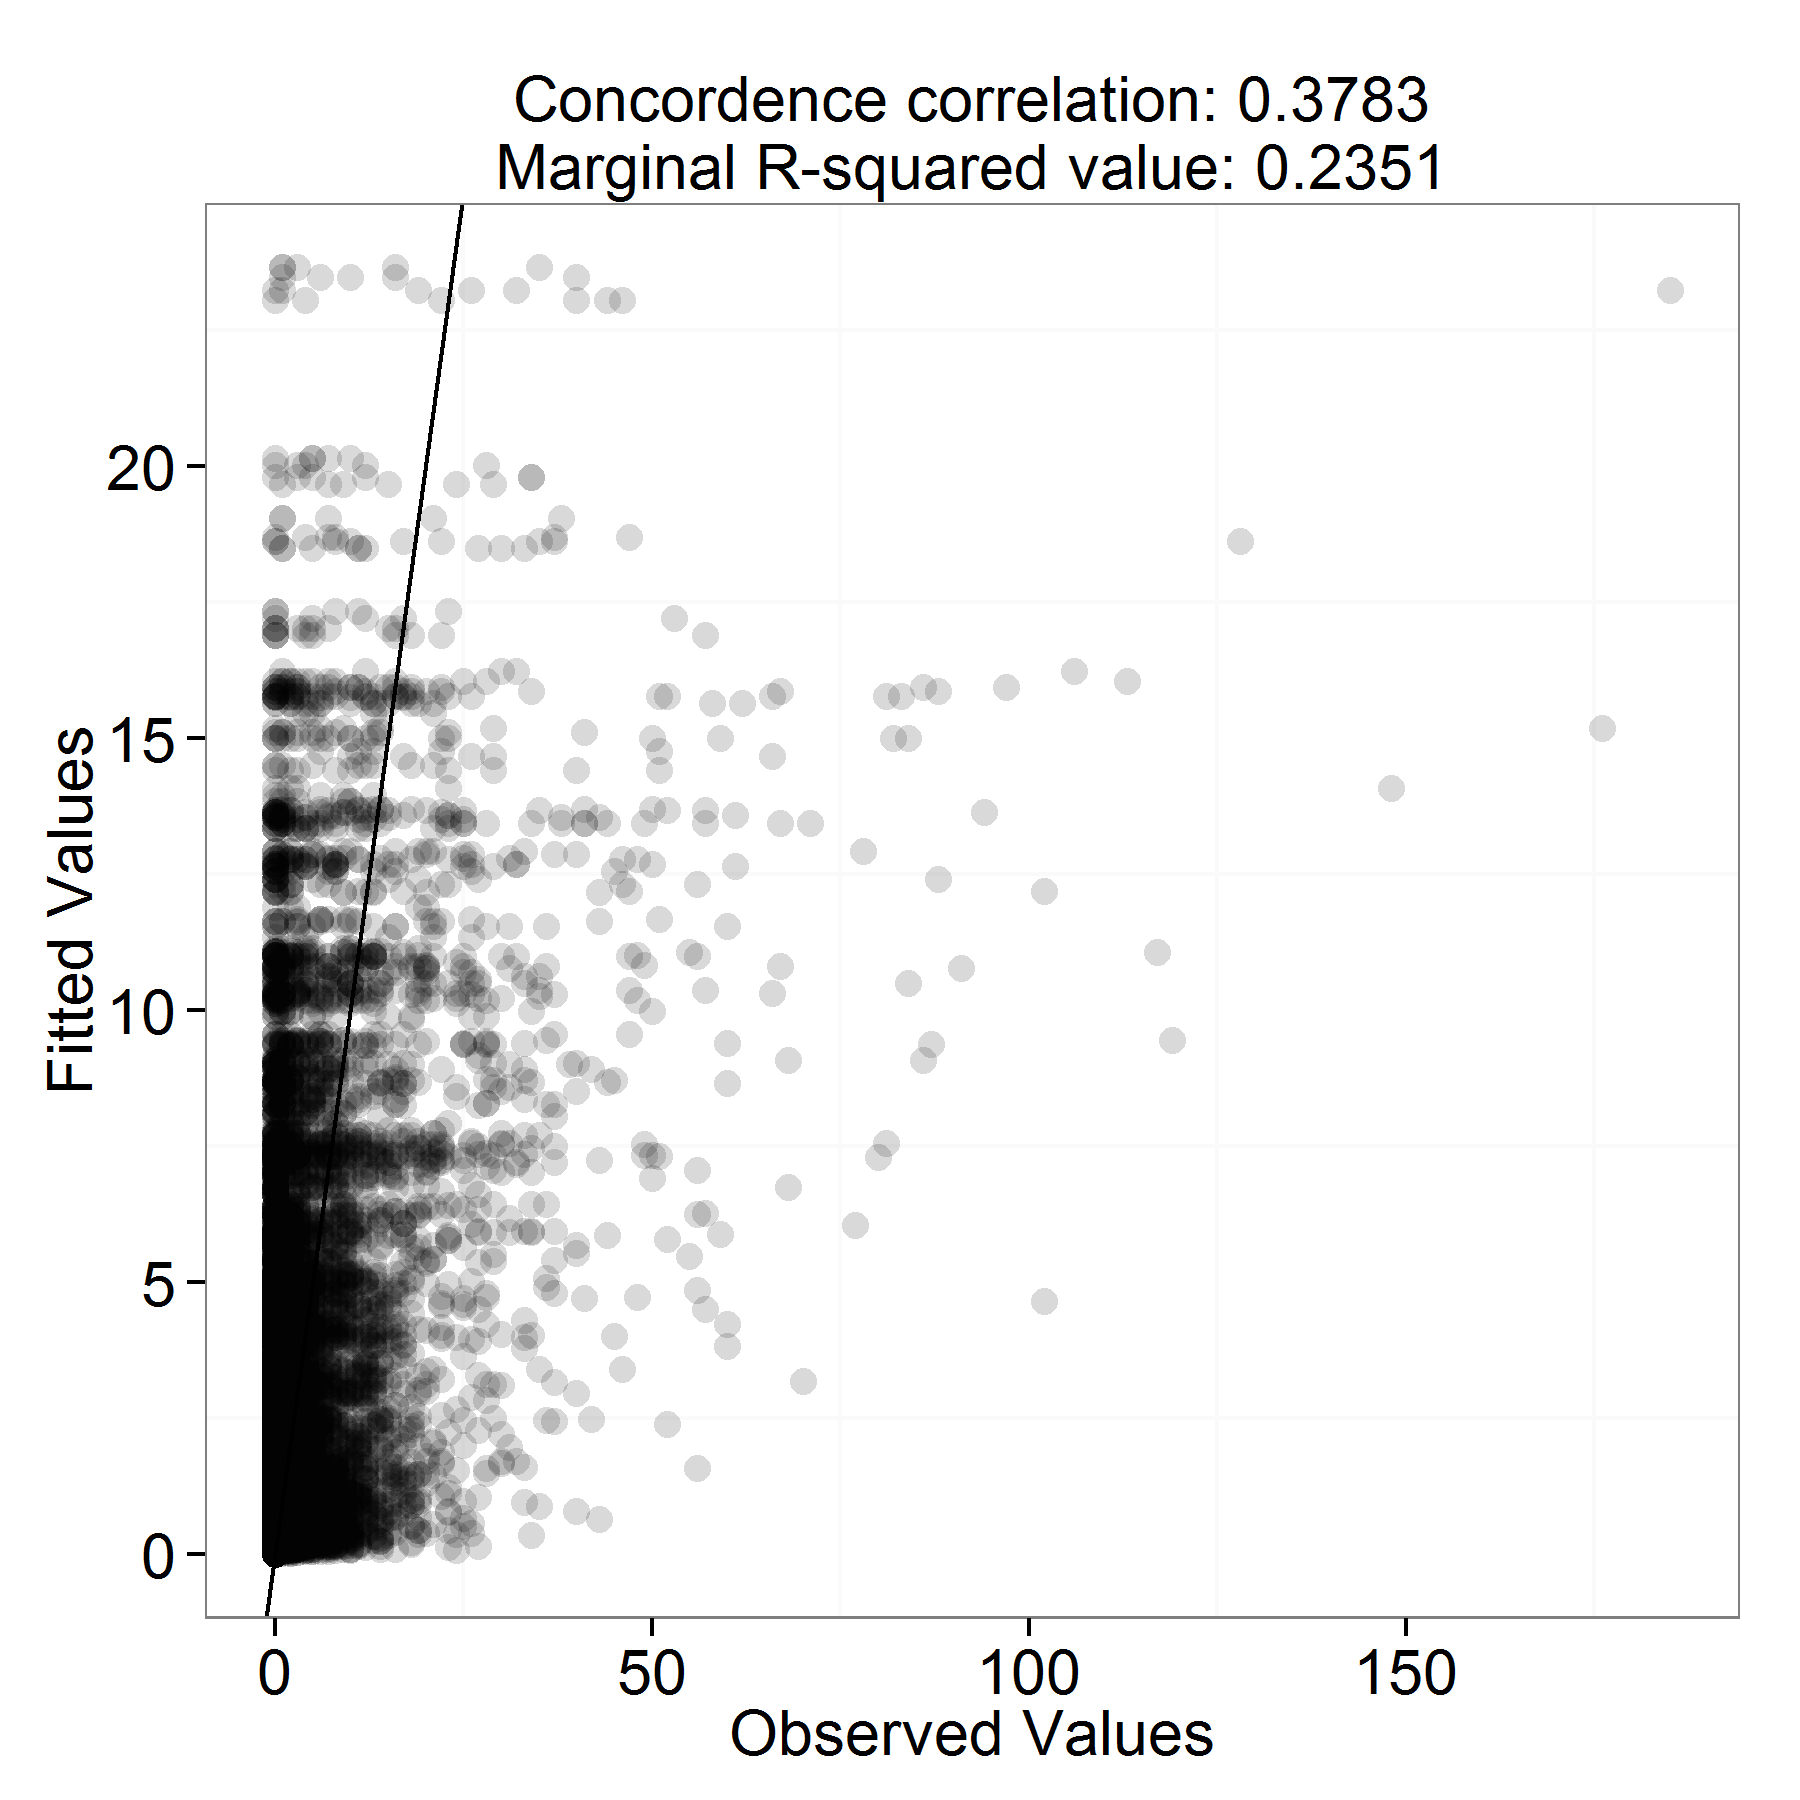
\includegraphics[width=7cm]{bc/FitPlots_fitted.png}
  \caption{Diagnostic plots of observed vs fitted values, where the diagonal line indicates where data should lie for a perfect fit.}
  \label{fig:nsdiagplots1}
\end{figure}
\end{frame}

\begin{frame}
\frametitle{Observed vs fitted}
\begin{itemize}
\item High observed values are under-predicted (Figure \ref{fig:nsdiagplots1})
\item Observed zeros tend to be over-predicted  (as is likely given they cannot be under-predicted)
\item Marginal R-squared and concordance correlation are low
\pause
\bigskip
\item Conclusion: poor model fit
\end{itemize}
\end{frame}

%~~~~~~~~~~~~~~~~~~~~~~~~~~~~~~~~~~~~~~~~~~~~~~~~~~
%~~~~~~~~~~~~~~~~~~~~~~~~~~~~~~~~~~~~~~~~~~~~~~~~~~~~~

\begin{frame}[fragile]
\frametitle{Fitted values vs scaled Pearsons residuals Plot}
The plot gives an indication of the correct mean-variance relationship assumed under the model.  We expect to see no pattern in the plot.  

\begin{itemize}
\item For a Poisson model the size of residuals is expected to increase with increasing fitted values
\item For overdispersed data the size of residuals increases at a faster rate than the strict Poisson relationship
\item To get a plot with an expectation of no pattern we use Pearsons residuals to account for the former and scaled these by the dispersion parameter (estimated by {\tt geeglm}) for the latter
\item Thus we plot Fitted values against scaled Pearsons residuals
\end{itemize}
\end{frame}

\begin{frame}[fragile]
\begin{figure}[h]
  \centering
    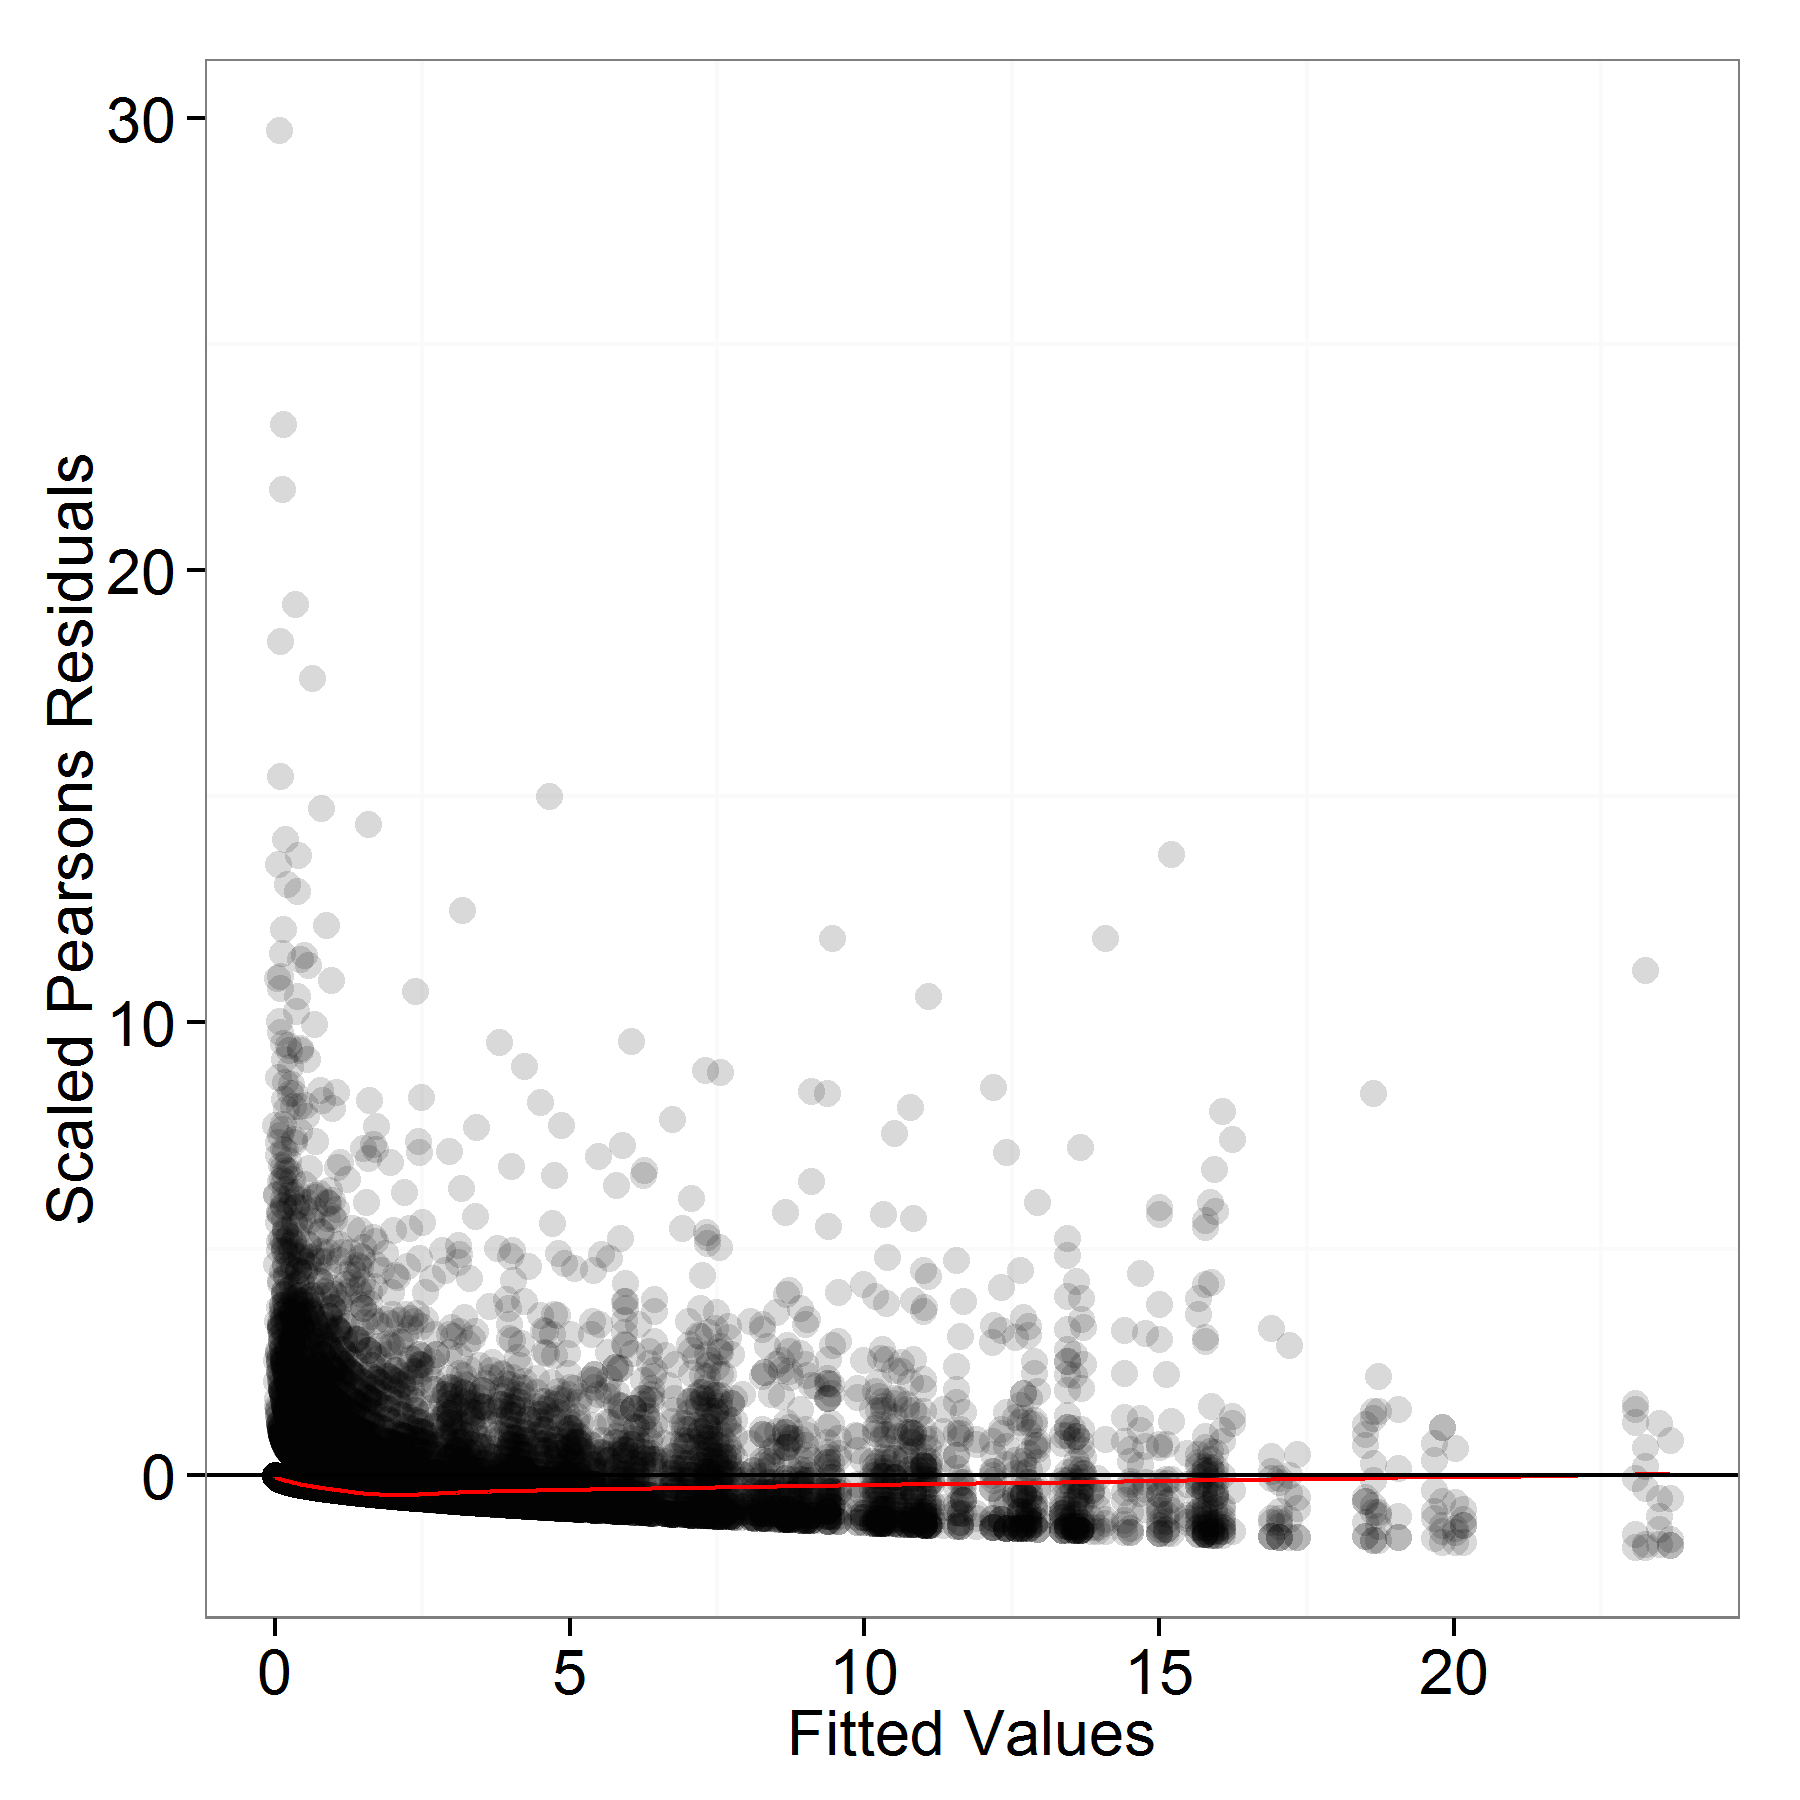
\includegraphics[width=7cm]{bc/FitPlots_resids.png}
  \caption{Diagnostic plot of fitted values vs scaled Pearsons residuals, where the red line is a locally weighted least squares regression to indicate pattern in the plot, which might otherwise be hidden due to over-plotting.}
  \label{fig:nsdiagplots2}
\end{figure}
\end{frame}

\begin{frame}
\begin{itemize}
\item Possible pattern in residuals but hard to tell due to overplotting (Figure \ref{fig:nsdiagplots2})
\item Locally weighted least squares regression line does not indicate an unusual pattern
\pause
\bigskip
\item Conclusion: no issue with model assumption (mean-variance relationship)
\end{itemize}
\end{frame}

%~~~~~~~~~~~~~~~~~~~~~~~~~~~~~~~~~~~~~~~~~~~~~~~~~~
%~~~~~~~~~~~~~~~~~~~~~~~~~~~~~~~~~~~~~~~~~~~~~~~~~~~~~
\subsection{Cumulative Residuals and runs profiles}

\begin{frame}[fragile]
\begin{itemize}
\item Assessment of systematic over- or under- prediction using cumulative residuals.
\item Assessment of the correlated nature of the residuals (how random they are) given that the residuals are ordered by covariate value, predicted value or temporally.
\end{itemize}

\begin{knitrout}\footnotesize
\definecolor{shadecolor}{rgb}{0.969, 0.969, 0.969}\color{fgcolor}\begin{kframe}
\begin{alltt}
\hlfunctioncall{plotCumRes}(geeModel, varlist=\hlfunctioncall{c}(\hlstring{'observationhour'}), splineParams=splineParams, 
    d2k=dists)
\hlfunctioncall{plotRunsProfile}(geeModel, varlist=\hlfunctioncall{c}(\hlstring{'observationhour'}))
\end{alltt}
\end{kframe}
\end{knitrout}

\end{frame}

\begin{frame}[fragile]
\frametitle{Cumulative residuals and runs profiles for observation hour}
\begin{figure}[h!]
  \centering
\subfloat[]{
  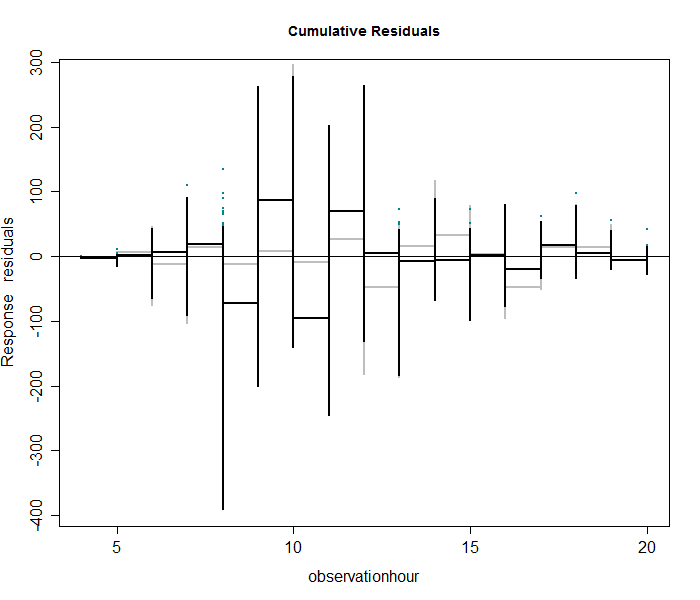
\includegraphics[width=6cm]{bc/CumRes_observationhour_gee.png}
}
\subfloat[]{
	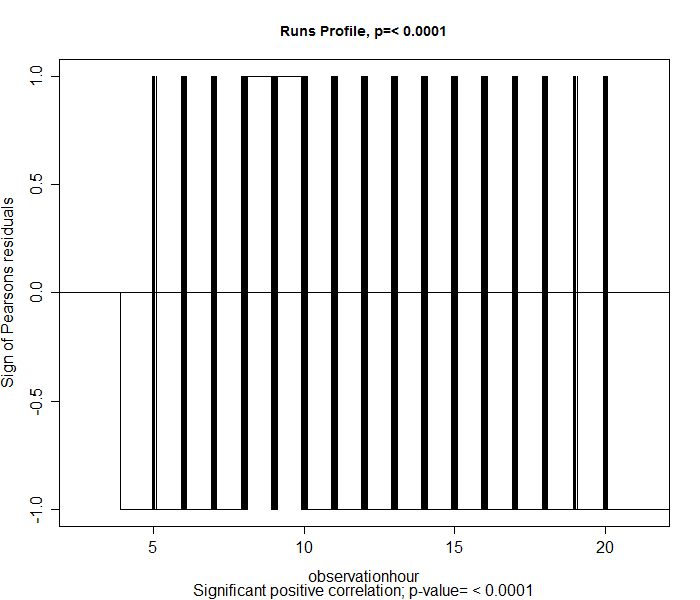
\includegraphics[width=6cm]{bc/RunsProfile_observationhour_gee.png}
}
    \caption{Cumulative residual plot (a) and runs profile (b) for residuals ordered by observation hour. The blue points are the residual values, the black line represents the cumulative residuals. The grey line in the background is what we would expect the cumulative residuals to be if observation hour was modelled correctly.}
  \label{fig:nsgeeruns1}
\end{figure}
\end{frame}

\begin{frame}[fragile]
Ordered by \textbf{observation hour}
\begin{itemize}
\item No systematic over or under prediction (Figure \ref{fig:nsgeeruns1})
\item Variable modelled appropriately:
\begin{itemize}
  \item similar to expected relationship (grey line) and better than Figure \ref{fig:nscumres1}
  \item good mixing about the zero cumulative residual line
\end{itemize}
\item Discrete nature of variable makes inference (visual) difficult
\item Visually good mixing, but fewer runs than would be expected if residuals were random ($p<<0.05$)
\item Significant positive correlation between residuals when ordered by observation hour
\end{itemize}
\end{frame}

\begin{frame}[fragile]
\frametitle{Cumulative residuals and runs profiles ordered by predicted value}
\begin{figure}[h!]
  \centering
    \subfloat[]{
  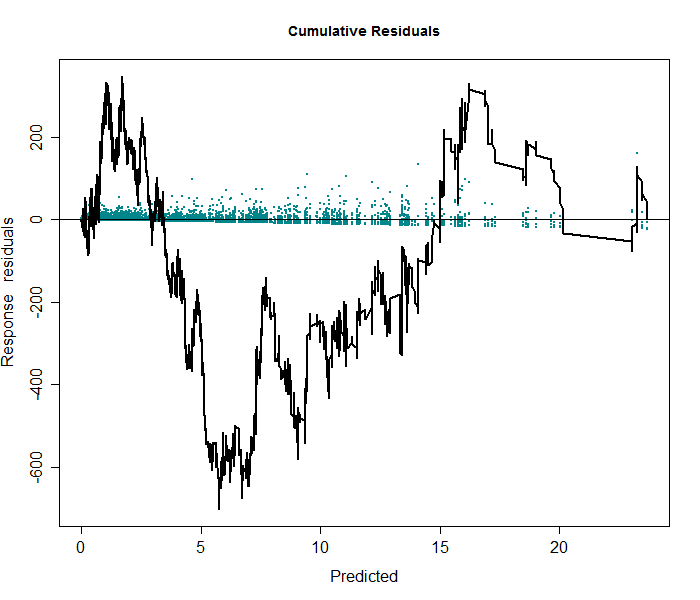
\includegraphics[width=6cm]{bc/CumRes_Predicted_gee.png}
}
\subfloat[]{
	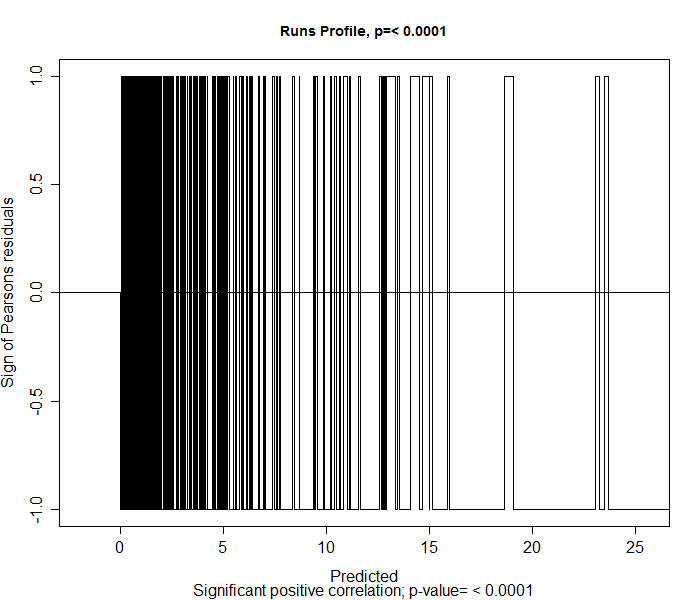
\includegraphics[width=6cm]{bc/RunsProfile_Predicted_gee.png}
}
    \caption{Cumulative residual plot (a) and runs profile (b) for residuals ordered by the predicted value.  The blue points are the residual values and the black line represents the cumulative residuals.}
  \label{fig:nsgeeruns2}
\end{figure}
\end{frame}

\begin{frame}[fragile]
Ordered by \textbf{prediction} value
\begin{itemize}
\item Under prediction at predicted density $< 3$ (Figure \ref{fig:nsgeeruns2})
\item Over-predicted up to about 12 birds/km$^2$
\item Thereafter some over/under prediction
\item But, fewer runs than would be expected if residuals were random ($p<0.05$)
\item Significant positive correlation between residuals when ordered by predicted value
\end{itemize}
\end{frame}

\begin{frame}[fragile]
\frametitle{Cumulative residuals and runs profiles ordered temporally}  
\begin{figure}[h!]
  \centering
  \subfloat[]{
  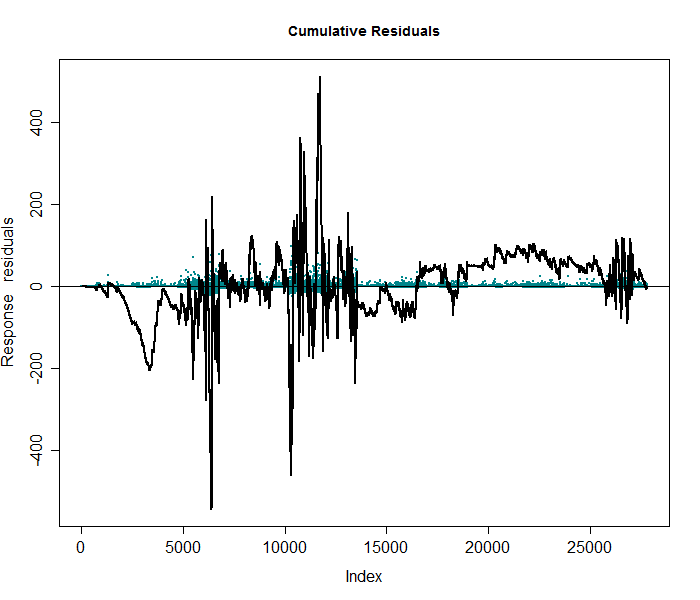
\includegraphics[width=6cm]{bc/CumRes_Index_gee.png}
}
\subfloat[]{
	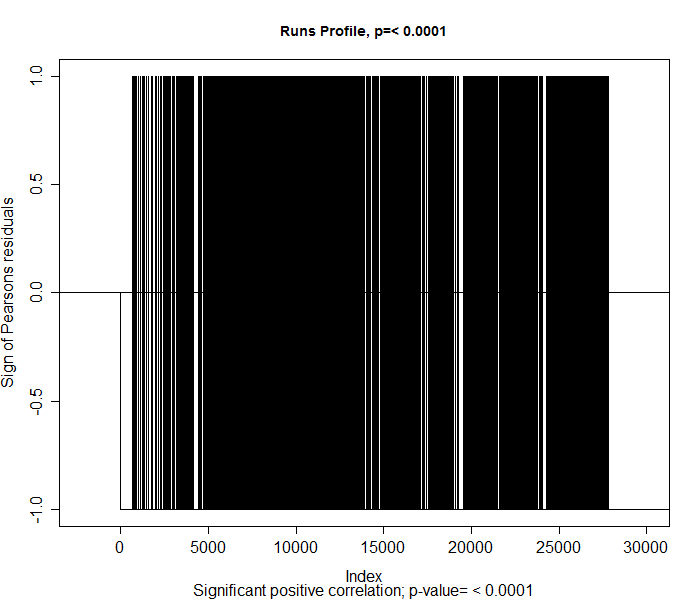
\includegraphics[width=6cm]{bc/RunsProfile_Index_gee.png}
}
  \caption{Cumulative residual plot (a) and runs profile (b) for residuals ordered by the index of observations (temporally).  The blue points are the residual values and the black line represents the cumulative residuals.}
  \label{fig:nsgeeruns3}
\end{figure}
\end{frame}


\begin{frame}[fragile]
Ordered by \textbf{index} (temporally)
\begin{itemize}
\item Lot of mixing about zero cumulative residual line (Figure \ref{fig:nsgeeruns3})
\item Best mixing of residuals seen in the runs profile 
\item But, still fewer runs than would be expected if residuals were random ($p<0.05$)
\item Significant positive correlation between residuals when ordered temporally
\end{itemize}
\end{frame}

\begin{frame}
\frametitle{Cumulative residuals and Runs Profiles}
\begin{itemize}
  \item Despite the inclusion of temporal covariates (tidal state and impact) we still have some unmodelled correlation
  \item We model this correlation using GEEs
  \item $p$-values from ANOVA (fitted earlier to decide which covariates to keep) are reliable due to modelled correlation
\end{itemize}


\end{frame}
% ~~~~~~~~~~~~~~~~~~~~~~~~~~~~~~~~~~~~~~~##
% ~~~~~~~~~~~~~~~~~~~~~~~~~~~~~~~~~~~~~~~##

\subsection{COVRATIO and PRESS statistics}

\begin{frame}[fragile]
The PRESS and COVRATIO statistics are relative measures that assess how aspects of the model change when individual blocks are removed from the analysis.

\begin{block}{COVRATIO statistic}
Signals the change in the \textbf{precision of the parameter estimates} when each block is omitted. 
\end{block}
\end{frame}

\begin{frame}[fragile]
\begin{block}{PRESS statistic}
Quantifies the sensitivity of \textbf{model predictions} to removing each block. 
\end{block}

\pause
\bigskip
\noindent See section \ref{subsec:covpress} for more details on COVRATIO and PRESS statistics.
\end{frame}

\begin{frame}[fragile]
\begin{knitrout}\footnotesize
\definecolor{shadecolor}{rgb}{0.969, 0.969, 0.969}\color{fgcolor}\begin{kframe}
\begin{alltt}
\hlfunctioncall{timeInfluenceCheck}(geeModel, data$blockid, dists, splineParams)
\hlcomment{# influence plots (covratio and press statistics)}
influence <- \hlfunctioncall{runInfluence}(geeModel, data$blockid, dists, splineParams)
\end{alltt}
\end{kframe}
\end{knitrout}
\end{frame}

\begin{frame}[fragile]
\begin{figure}[h]
  \centering
  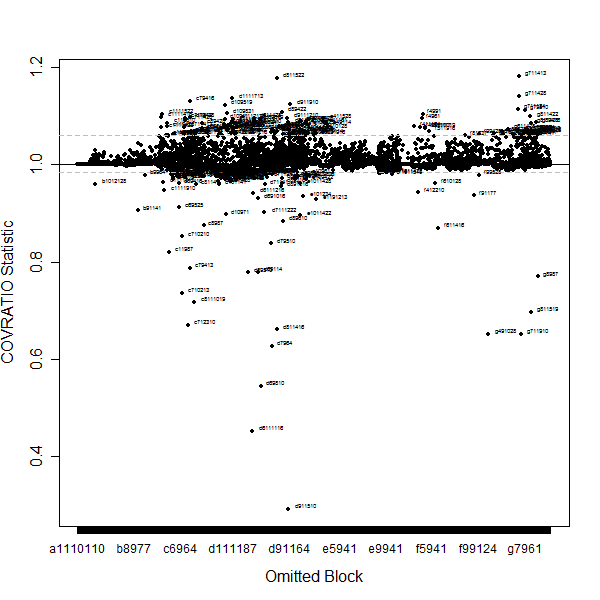
\includegraphics[width=7cm]{bc/InfluenceMeasures_covratio.png}
  \caption{Plot of COVRATIO statistics; the dashed grey lines indicate the lower 2.5\% and upper 97.5\% quantiles of the statistics.}
  \label{fig:nsinfluence1}
\end{figure}
\end{frame}

\begin{frame}[fragile]
\frametitle{COVRATIO statistics}
\begin{itemize}
  \item there will always be blocks outside the dashed lines (they are quantiles)
  \item As it is a relative measure, blocks far away may be of concern
  \item Blocks with COVRATIO statistic $< 1$ are of most concern (decrease in precision when removed) 
  \item Here, blocks {\tt d611810} and {\tt d6111116} are far away and result in an decrease in standard errors when removed (Figure \ref{fig:nsinfluence1})
  \item These blocks are both grid code {\tt D6} in the year 2011 (first of two years after impact) and the former in month 8 and the 10$^{\textrm{th}}$ day of the month.  
  \item Both blocks have particularly high bird counts compared with most blocks and so adds to the variability in the data.
  \bigskip
  \item Conclusion: Variability increases with higher counts for Poisson data and so it is fine for these blocks to remain. 
  \end{itemize}
\end{frame}

% ~~~~~~~~~~~~~~~~~~~~~~~~~~~~~~~~~~~~~~~##
% ~~~~~~~~~~~~~~~~~~~~~~~~~~~~~~~~~~~~~~~##
\begin{frame}[fragile]
\begin{figure}[h]
  \centering
    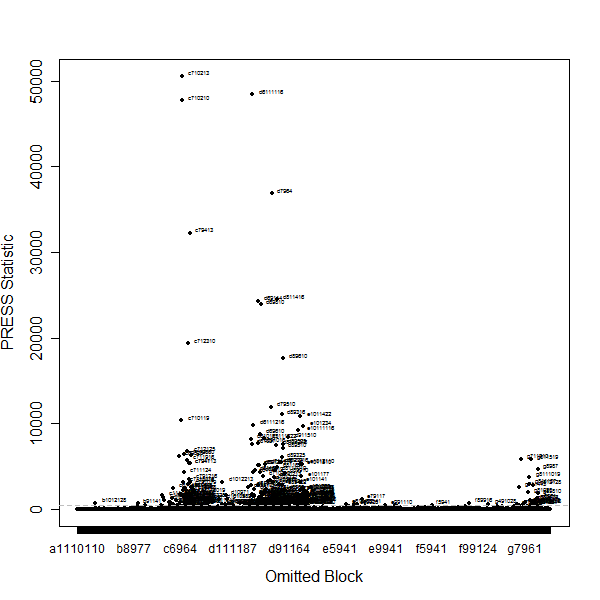
\includegraphics[width=7cm]{bc/InfluenceMeasures_press.png}
  \caption{Plot of PRESS statistics; 95\% of the statistics fall below the dashed grey lines.  Labelled points on both plots are outside the grey dashed line(s) and are labelled with the identifier for the block that has been removed to create the statistic (not an observation number).}
  \label{fig:nsinfluence2}
\end{figure}
\end{frame}


\begin{frame}
\frametitle{PRESS statistics}
\begin{itemize}
  \item there will always be blocks above the dashed line (it is a quantile)
  \item As it is a relative measure, blocks far away may be of concern
  \item Predictions are sensitive to several blocks: {\tt c710213} {\tt c710210} and {\tt d6111116} (Figure \ref{fig:nsinfluence2}).
  \item As above, these blocks all contain very high bird counts  
  \bigskip
  \item Conclusion: Variability increases with higher counts for Poisson data and so it is fine for these blocks to remain. 
\end{itemize}
\end{frame}

% ~~~~~~~~~~~~~~~~~~~~~~~~~~~~~~~~~~~~~~~##
% ~~~~~~~~~~~~~~~~~~~~~~~~~~~~~~~~~~~~~~~##
\subsection{Raw Residuals}
\begin{frame}[fragile]
Raw residuals (observed - fitted values) can be represented spatially to ascertain if some areas are over/under predicted.  

\begin{itemize}
\item No real spatial pattern to the residuals (Figure \ref{fig:nsrawresid})
\item No systematic over/under prediction
\bigskip
\item Conclusion: No spatial bias in model
\end{itemize}
\end{frame}

\begin{frame}[fragile]
\begin{figure}[h]
  \centering
  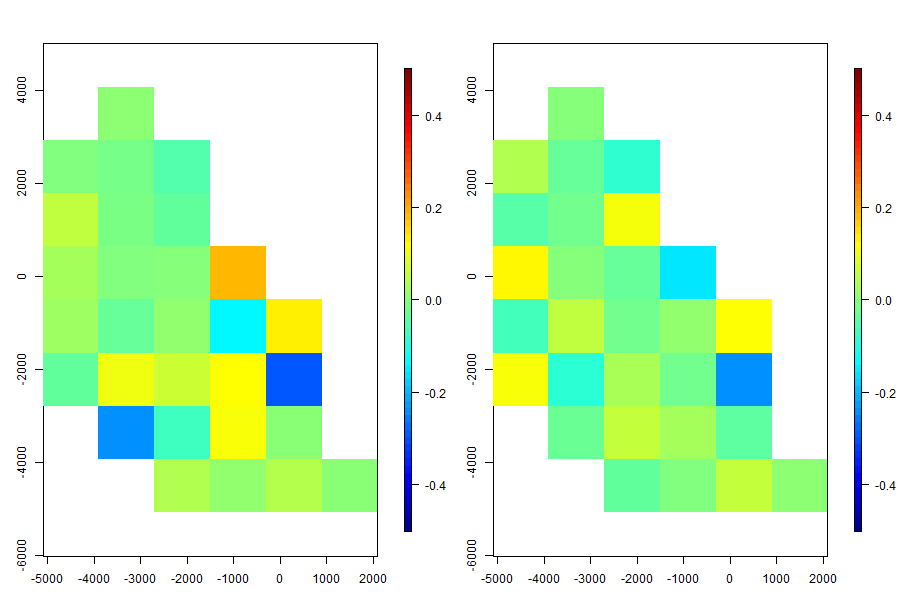
\includegraphics[width=12cm]{bc/residualPlot.png}
  \caption{Raw residuals before impact (left) and after impact (right). These residuals are fitted values - observed values (mean$^*$ birds/km$^2$). $^*$ mean density because the predictions are for several observation hours.}
  \label{fig:nsrawresid}
\end{figure}
\end{frame}

\begin{frame}[fragile]
\frametitle{}
\begin{knitrout}\footnotesize
\definecolor{shadecolor}{rgb}{0.969, 0.969, 0.969}\color{fgcolor}\begin{kframe}
\begin{alltt}
\hlcomment{# residual plot}
resids <- \hlfunctioncall{fitted}(geeModel) - data$birds
dims <- \hlfunctioncall{getPlotdimensions}(data$x.pos, data$y.pos, 1000, 1000)

\hlfunctioncall{par}(mfrow = \hlfunctioncall{c}(1, 2), mar = \hlfunctioncall{c}(3, 3, 3, 5))
\hlfunctioncall{quilt.plot}(data$x.pos[data$impact == 0], data$y.pos[data$impact == 
    0], resids[data$impact == 0], asp = 1, ncol = dims[2], nrow = dims[1], 
    zlim = \hlfunctioncall{c}(-2.2, 2.2))
\hlfunctioncall{quilt.plot}(data$x.pos[data$impact == 1], data$y.pos[data$impact == 
    1], resids[data$impact == 1], asp = 1, ncol = dims[2], nrow = dims[1], 
    zlim = \hlfunctioncall{c}(-2.2, 2.2))
\end{alltt}
\end{kframe}
\end{knitrout}

\end{frame}

\clearpage
\begin{frame}
\frametitle{How did we do?}
\begin{table}[h]
\centering
\scriptsize
\caption{Table of potential modelling problems, what method was used to assess the problem, was the potential problem an issue in reality and if yes then what was the solution.  Solutions in red were not done and are possibilities for the future.}
\begin{tabular}{l|c|c|c}
\textbf{} & \textbf{Method} & \textbf{Issue (Y/N)} & \textbf{Solution}\\
\hline
Collinearity & VIF & N & -\\
Over-dispersion& - & Y & estimated by GEE\\
Model Fit & Observed vs Fitted & Y & {\color{red} use more covariates}\\
mean-variance relationship & Fitted vs residuals & N & -\\
Correlated Residuals & runs test & Y & modelled by GEE\\
Correlated Residuals & Runs profile & Y & modelled by GEE\\
Covariate specification & cumulative residuals & N & -\\
systematic over/under prediction & cumulative residuals & N & -\\
spatial systematic over/under prediction & raw residual plot & N & -\\
removing blocks & COVRATIO statistics & N & - \\
removing blocks & PRESS statistics & N & - \\

\end{tabular}
\label{tab:fitstats}
\end{table}

\end{frame}

%~~~~~~~~~~~~~~~~~~~~~~~~~~~~~~~~~~~~~~~~~
%~~~~~~~~~~~~~~~~~~~~~~~~~~~~~~~~~~~~~~~~~~~
\markedsection{Preds \& Inference}{Prediction and Inference}
\label{sec:nspreds}

\subsection{Data requirements for predicting}
For making predictions, we require a data frame containing grid data with records for which to make predictions. This requires certain columns and records these can be summarised as:\\
\large
\begin{itemize}
\item{\textbf{Columns:} each covariate retained in the best fitting model with exactly matching column names}
\item{\textbf{Columns:} \textit{x.pos} and \textit{y.pos} provide geographic position information used for calculating distance matrices for CReSS/SALSA}
\item{\textbf{Columns:} \textit{area} provides the area of each grid cell. }
\item{\textbf{Rows:} 1 record for each grid cell and for each date and time a prediction is made for}
\end{itemize}

%\begin{frame}[fragile]
\noindent Using our case study of nearshore data, we have a look at our prediction data using the \textit{head} function after we load the data. 
\begin{knitrout}\footnotesize
\definecolor{shadecolor}{rgb}{0.969, 0.969, 0.969}\color{fgcolor}\begin{kframe}
\begin{alltt}
\hlcomment{# loading the prediction grid data}
\hlfunctioncall{data}(ns.predict.data.re)
predictData <- ns.predict.data.re
\hlfunctioncall{head}(predictData)
\end{alltt}
\begin{verbatim}
  x.pos y.pos     area floodebb observationhour GridCode Year DayOfMonth
1  1500 -4500 0.385253      EBB              12      a11    9         13
2  1500 -4500 0.385253    FLOOD               8      a11    9         16
3  1500 -4500 0.385253    FLOOD               9      a11    9         16
4  1500 -4500 0.385253    FLOOD              10      a11    9         16
5  1500 -4500 0.385253    FLOOD              11      a11    9         16
6  1500 -4500 0.385253    FLOOD              12      a11    9         16
  MonthOfYear impact        truth
1           3      0 0.0003871928
2           3      0 0.0006163433
3           3      0 0.0006064698
4           3      0 0.0005072918
5           3      0 0.0004220902
6           3      0 0.0003570533
\end{verbatim}
\end{kframe}
\end{knitrout}

\noindent Note: the {\tt truth} column is an artefact of this being simulated data.   Ordinarily the user would not know this.


\subsection{Making predictions}
\label{ss:predictions}
\noindent We make predictions using our best fitting CReSS/SALSA model from the previous sections. This requires three steps: 
\begin{enumerate}
\item{Creating a matrix of distances from the prediction data to knots}
\item{Making predictions to the prediction data using the best fitting model}
\item{Converting the predictions back to the response scale}
\end{enumerate}

\begin{knitrout}\footnotesize
\definecolor{shadecolor}{rgb}{0.969, 0.969, 0.969}\color{fgcolor}\begin{kframe}
\begin{alltt}
\hlcomment{# create the distance matrix for predictions }
dists <- \hlfunctioncall{makeDists}(\hlfunctioncall{cbind}(predictData$x.pos, predictData$y.pos), 
    \hlfunctioncall{na.omit}(knotgrid), knotmat = FALSE)$dataDist
\hlcomment{# use baseModel to make predictions to avoid a warning from }
\hlcomment{# using geeModel (same answers though)}
predslink <- \hlfunctioncall{predict}(baseModel, predictData, type = \hlstring{"link"})
\hlcomment{# reversing the log-link to convert predictions back to the response scale}
preds <- \hlfunctioncall{exp}(predslink)
\end{alltt}
\end{kframe}
\end{knitrout}
\noindent The object {\tt preds} contains the predictions for each record in our prediction grid. 

\subsection{Visualising the redistribution using predictions}
\noindent We know that our model identified a redistribution of animals within the study area by the significant interaction term between impact and the two-dimensional smooth of {\tt x.pos} and {\tt y.pos}. From the model coefficients it is not obvious where the redistribution has occurred. We are going to investigate this by visualising the redistribution using our predictions. 

\noindent The following is code for plotting the model predictions in Figure \ref{fig:nspointest}.
\begin{knitrout}\footnotesize
\definecolor{shadecolor}{rgb}{0.969, 0.969, 0.969}\color{fgcolor}\begin{kframe}
\begin{alltt}
\hlcomment{# plotting the predictions for before and after impact}
\hlcomment{# get the plot dimensions. We know each cell is 1000x1000m}
dims<-\hlfunctioncall{getPlotdimensions}(x.pos=predict.data.re$x.pos, predict.data.re$y.pos, 
   segmentWidth=1000, segmentLength=1000)
\hlfunctioncall{par}(mfrow=c(1,2), mar=c(3,3,3,5))
\hlfunctioncall{quilt.plot}(predictData$x.pos[predictData$impact==0], 
    predictData$y.pos[predictData$impact==0], 
    preds[predictData$impact==0], asp=1, nrow=dims[1], ncol=dims[2], 
    zlim=c(0, maxlim))
\hlfunctioncall{quilt.plot}(predictData$x.pos[predictData$impact==1], 
    predictData$y.pos[predictData$impact==1], preds[predictData$impact==1], 
    asp=1,nrow=dims[1], ncol=dims[2], zlim=c(0, maxlim))
\end{alltt}
\end{kframe}
\end{knitrout}
\noindent Note that the value for {\tt maxlim} can be determined by plotting both plots without the {\tt zlim} argument first from which you can determine what the maximum value in the scale of either plot is. 
\begin{block}{The quilt.plot function}
\begin{itemize}
\item{Plots averages of the predictions for each grid cell}
\item{Subsetting the data using the square brackets restricts the input data to before (left) and after impact (right plot)}
\item{Using the {\tt zlim} argument allows ensuring that left and right plot have the same scale colour scheme. }
\item{The dimensions of the plot ({\tt nrow} and {\tt ncol}) determine the size of each grid cell.  Since we know our grid to be 1000m by 1000m we can use {\tt getPlotDimensions} to find the values for these arguments.}
\end{itemize}
\end{block}

\begin{figure}[h]
  \centering
  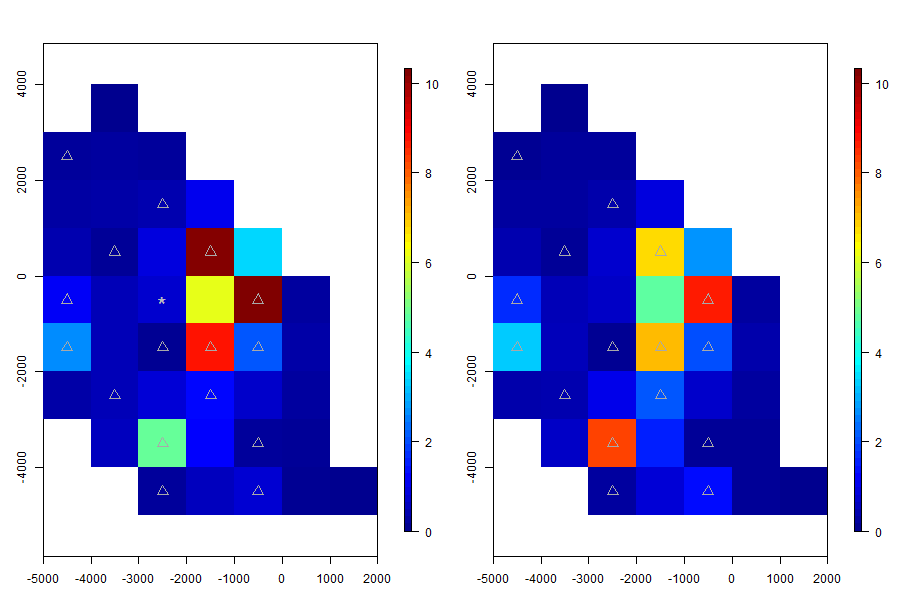
\includegraphics[width=12cm]{bc/pointEstimate.png}
  \caption{Predictions of bird density (mean birds/km$^2$) from the fitted model for before (left) and after (right) an impact event. The * indicated the location of the impact; the $\triangle$ indicate the knot locations.}
  \label{fig:nspointest}
\end{figure}
\begin{block}{Conclusion}
\begin{itemize}
  \item Decline in bird density in the central eastern region
  \item Increase in density in the south of the study region 
  \item The central region is where a known impact has taken place and the results suggest that birds have moved from this region to the south after the impact event
\end{itemize}
\end{block}

\begin{block}{Next step}
\begin{itemize}
  \item Is this difference real or simply random noise?
  \item We need to classify if the differences are significant or due to sampling variation.
  \item We do this by constructing bootstrap confidence intervals for each prediction in the prediction grid data.
\end{itemize}
\end{block}
%\end{frame}

% ~~~~~~~~~~~~~~~~~~~~~~~~~~~~~~~~~~~~~~~~~~~~~~

\markedsection{Bootstrap CIs}{Bootstrap confidence intervals}
%\begin{frame}[fragile]
\noindent Following the predictions from section \ref{ss:predictions}, we now create replicate predictions and use these to construct percentile confidence intervals around each prediction grid cell. We run {\tt B} iterations performing the following: 
\begin{itemize}
\item Input best model from fitting to the original observed data.
\item{Use the model coefficients and covariance matrix to sample new coefficients from a multivariate Normal distribution.}
\item{Make predictions to the study area using these coefficients.}
\end{itemize}
This approach incorporates the uncertainty associated with the count model coefficients. 
%\end{frame}

\begin{block}{The {\tt do.bootstrap.cress} function}
This function performs the number of bootstrap iterations specified with the argument {\tt B} where the fitting model is CReSS. The recommended number of bootstrap iterations is 999. \\

If {\tt ddf.obj} is set to {\tt NULL}, this function automatically applies the 'no distance sampling'-approach with the three steps described above.\\

Since the prediction object can be quite large, it is not returned but saved to file in the current working directory with the file name `predictionboot.RData'.  
\end{block}

\begin{knitrout}\footnotesize
\definecolor{shadecolor}{rgb}{0.969, 0.969, 0.969}\color{fgcolor}\begin{kframe}
\begin{alltt}
\hlcomment{# do the bootstrap}
\hlfunctioncall{do.bootstrap.cress}(data, predictData, ddf.obj=NULL, baseModel, splineParams, 
                dists, B=250)
\end{alltt}
\end{kframe}
\end{knitrout}

\noindent In the next step we use these bootstrap predictions to construct our 95\% confidence intervals for each prediction. 

\begin{block}{The {\tt makeBootCIs} function}
Using the {\tt B} bootstrap predictions from a call to the {\tt do.bootstrap.cress} function, the {\tt makeBootCIs} function creates lower and upper limits for 95\% confidence intervals using the percentile method for each record in the prediction data. \\

\noindent An optional argument {\tt quants} can be used to specify an interval other than 95\%.  The default is {\tt quants = c(0.025, 0.975)}
\end{block}

\begin{knitrout}\footnotesize
\definecolor{shadecolor}{rgb}{0.969, 0.969, 0.969}\color{fgcolor}\begin{kframe}
\begin{alltt}
\hlcomment{# read in bootstrap predictions}
\hlfunctioncall{load}("predictionboot.RData")
\hlcomment{# make percentile confidence intervals}
cis <- \hlfunctioncall{makeBootCIs}(bootPreds)
\end{alltt}
\end{kframe}
\end{knitrout}


\subsection{Visualising bootstrap confidence intervals}

Figure \ref{fig:nscis} depicts the range of uncertainty in the spatial estimates of density.  These can be contrasted with the point estimates found in Figure \ref{fig:nspointest}.

In this section we will investigate whether looking at the lower and upper confidence limits from the 95\% confidence intervals will give us a similar picture as looking at the predictions. 
%\begin{knitrout}\footnotesize
%\definecolor{shadecolor}{rgb}{0.969, 0.969, 0.969}\color{fgcolor}\begin{kframe}
%\begin{alltt}
%\hlcomment{# plotting the confidence intervals for before and after impact}
%\hlfunctioncall{par}(mfrow=c(2,2), mar=c(3,3,3,5))
%\hlfunctioncall{quilt.plot}(predictData$x.pos[predictData$impact==0], 
%predictData$y.pos[predictData$impact==0], 
%cis[predictData$impact==0,2], asp=1, nrow=7, ncol=9, 
%zlim=c(0, maxlim))
%\hlfunctioncall{quilt.plot}(predictData$x.pos[predictData$impact==1], 
%predictData$y.pos[predictData$impact==1], cis[predictData$impact==1,2], 
%asp=1,nrow=7, ncol=9, zlim=c(0, maxlim))
%\hlfunctioncall{quilt.plot}(predictData$x.pos[predictData$impact==0], 
%predictData$y.pos[predictData$impact==0], 
%cis[predictData$impact==0,1], asp=1, nrow=7, ncol=9, 
%zlim=c(0, maxlim))
%\hlfunctioncall{quilt.plot}(predictData$x.pos[predictData$impact==1], 
%predictData$y.pos[predictData$impact==1], cis[predictData$impact==1,1], 
%asp=1,nrow=7, ncol=9, zlim=c(0, maxlim))
%\end{alltt}
%\end{kframe}
%\end{knitrout}


\begin{figure}[h!]
  \centering
  \subfloat{
  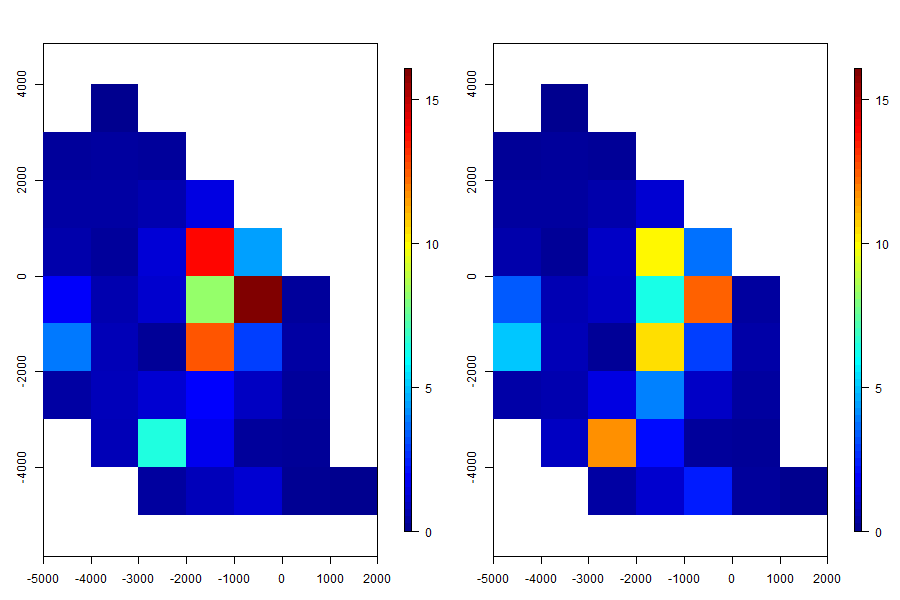
\includegraphics[width=9cm]{bc/cis_upper.png}
  }
  \hfill
  \subfloat{
    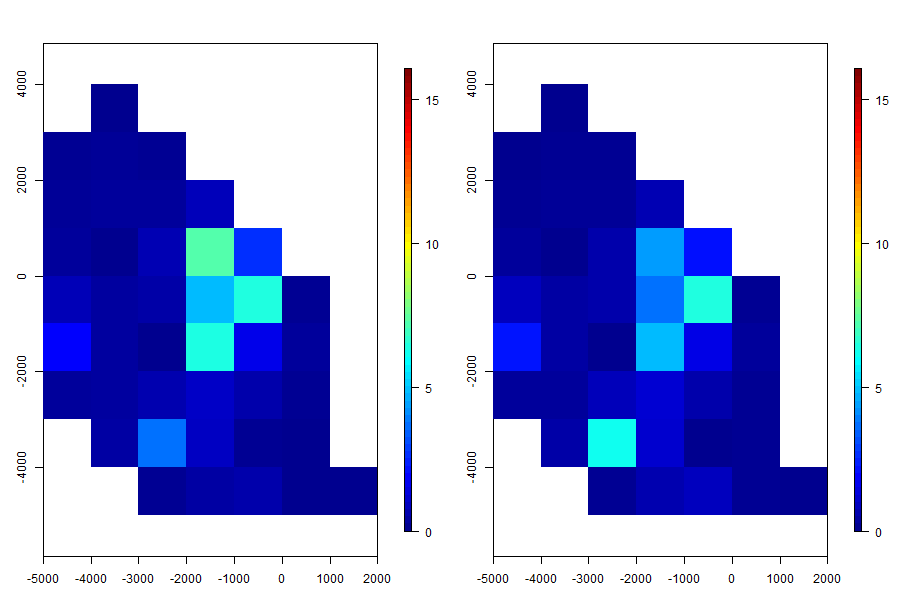
\includegraphics[width=9cm]{bc/cis_lower.png}
  }
  \caption{Upper (top) and lower (bottom) 95\% confidence intervals of bird density (birds/km$^2$) from the fitted model from before (left) and after (right) impact.}
  \label{fig:nscis}
\end{figure}

\begin{block}{Conclusion}
\begin{itemize}
  \item Lower and upper intervals before impact (left) show a higher density of birds in the central eastern region.  
  \item After impact (right), both lower and upper intervals show a decline in density in the central eastern region and an increase in the area to the south.  
  \item It is difficult to see where in the study region any significant differences may have occurred.
\end{itemize}
\end{block}


% ~~~~~~~~~~~~~~~~~~~~~~~~~~~~~~~~~~~~~~~~~~~~~~
\markedsection{Differences}{Identifying differences}
\noindent In this section we estimate the differences in predictions for each corresponding pair of records from our prediction grid. The first half of our prediction grid consists of records from before impact while the second half consists of records from after impact. \\

\noindent Note that the before and after data need to be ordered in the same manner and of the same length. 

\begin{block}{The {\tt getDifferences} function}
For each bootstrap iteration the differences in predictions from before and after impact are calculated (Density$_{after}$ - Density$_{before}$) and 95\% confidence intervals for the difference calculated using the percentile method. \\

\noindent If these intervals contain the value zero, a '0' is recorded. If they do not contain the value zero, '1' is recorded if the lower limit is above zero as an indication that the difference is significantly positive (increase in animal densities after impact). A '-1' is recorded if the upper limit is below zero, indicating that the difference is significantly negative (decrease in animal densities after impact). \\
The function returns a list of two objects: 
\begin{itemize}
\item{The median for each difference}
\item{The marker for significant positive and negative differences}
\end{itemize}
\end{block}


\begin{knitrout}\footnotesize
\definecolor{shadecolor}{rgb}{0.969, 0.969, 0.969}\color{fgcolor}\begin{kframe}
\begin{alltt}
differences <- \hlfunctioncall{getDifferences}(beforePreds = 
        bootPreds[predictData$impact == 0, ], 
        afterPreds = bootPreds[predictData$impact == 1, ])
\end{alltt}
\end{kframe}
\end{knitrout}


\subsection{Visualising significant differences}
To illustrate the differences in animal densities after impact, we plot the calculated differences (Density$_{after}$ - Density$_{before}$) using the {\tt quilt.plot} function.\\

\noindent The locations of the differences are added to the same plot using the '$\circ$' and '+' symbols. 
\begin{knitrout}\footnotesize
\definecolor{shadecolor}{rgb}{0.969, 0.969, 0.969}\color{fgcolor}\begin{kframe}
\begin{alltt}
\hlcomment{# The median for each after - before difference}
mediandiff <- differences$mediandiff
\hlcomment{# The marker for each after - before difference: 
positive ('1') and negative ('-1') significant differences}
marker <- differences$significanceMarker
\hlfunctioncall{par}(mfrow = \hlfunctioncall{c}(1, 1))
\hlfunctioncall{quilt.plot}(predictData$x.pos[predictData$impact == 0], 
    predictData$y.pos[predictData$impact ==  0], 
    mediandiff, asp = 1, nrow = 7, ncol = 9)
\hlcomment{# add + or - depending on significance of cells.  Just}
\hlcomment{# requires one significance out of all to be allocated}
\hlfunctioncall{points}(predictData$x.pos[predictData$impact==0][marker==1], 
    predictData$y.pos[predictData$impact==0][marker==1], pch=\hlstring{"+"}, 
    col=\hlstring{"darkgrey"},  cex=2)
\hlfunctioncall{points}(predictData$x.pos[predictData$impact==0][marker==(-1)], 
    predictData$y.pos[predictData$impact==0][marker==(-1)], col=\hlstring{"darkgrey"}, 
    cex=3)
\hlfunctioncall{points}(0,0,pch=20, col=\hlstring{"grey"},, cex=3)
\hlfunctioncall{points}(data$x.pos[which(data$GridCode=='e7')[1]], 
    data$y.pos[which(data$GridCode=='e7')[1]],cex=2, pch=\hlstring{"*"}, lwd=2, 
    col=\hlstring{"grey"})
\end{alltt}
\end{kframe}
\end{knitrout}

\begin{figure}[h]
  \centering
  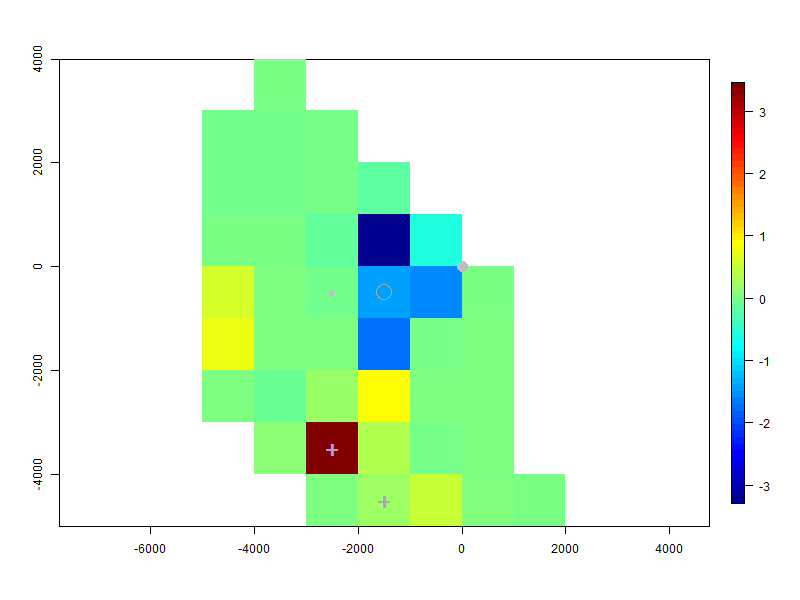
\includegraphics[width=8cm]{bc/differencePlot.png}
  \tiny
  \caption{Mean differences in predicted bird density (birds/km$^2$) before and after impact.  Positive values indicate more birds post impact and negative values fewer birds post impact.  Significant differences were calculated using percentile confidence intervals: '+' indicates a significant positive difference and '$\circ$' a significant negative one.  The grey star is the site of the impact event.}
  \label{fig:nsdiffs}
\end{figure}

\begin{block}{Conclusion}
 \begin{itemize}
  \item There was a significant decline in animals around the impact site and closest to the cliff-top observer (Figure \ref{fig:nsdiffs}).
  \item There was also a significant increase in animals in the south of the study area.
\end{itemize}
\end{block}

\markedsection{Comparison}{Comparison to the Truth}
Here we will finalise our analysis by comparing our results with the truth. This is possible as our data was simulated and hence the parameter values known. 
\subsection{Overdispersion and correlation}
We created data that were both overdispersed and positively correlated within any grid cell-day (i.e. observed counts from the same grid cell within the same day). 
\begin{table}[h!]
\begin{tabular}{l|r}
\textbf{Truth} & \textbf{Model}\\
\hline
Overdispersed  data & estimated overdispersion \\
 & parameter was greater than 1\\
\hline
Positively correlated data & accounted for using\\
 & GEE-based \textit{p}-values\\
\end{tabular}\end{table}
\begin{block}{Conclusion}
We conclude that our proposed methods are capable of identifying overdispersion and correlation in the data.
\end{block}

\subsection{Type of impact}
For this particular data set, the total number of animals before and after impact did not change. The type of impact that we implemented was a redistribution from the area surrounding the impact into the south of the study area. 
\begin{table}[ht!]
\begin{tabular}{l|r}
\textbf{Truth} & \textbf{Our model}\\
\hline
Redistribution  & identified with a \\
within study area & significant interaction term\\
\hline
Overall abundance  & identified with the non-significant \\
remained the same & main effect for impact\\
\end{tabular}
\end{table}
\begin{block}{Conclusion}
We conclude that our method was capable of correctly identifying the redistribution effect and reallocated birds to the correct locations despite highly correlated and overdispersed data. \\
\end{block}

%\end{document}
